\documentclass[asi]{picINSA}
\DeclareGraphicsRule{*}{pdf}{*}{}
\usepackage{pdfpages}
\usepackage{supertabular}

%\usepackage{colortbl}
\usepackage{fancyhdr}
\usepackage{listings} 
\usepackage{mathrsfs}
\usepackage{url}
\usepackage{lmodern}
\usepackage{color}
\usepackage{xcolor}
\usepackage{wrapfig}
\usepackage{graphicx}
\usepackage{pdflscape}
\usepackage{longtable}
\usepackage{sectsty}
\usepackage{lastpage}
\usepackage{multirow}
\usepackage{float}
\usepackage{eso-pic}
\usepackage[french]{minitoc}
\usepackage[babel=true]{csquotes}
\usepackage{tikz}
\addto\captionsfrench{\def\tablename{Tableau}}
\usepackage{../../ressources/Unipik/vocabulaire/vocabulaireUnipik}
%\usepackage{../../ressources/Unipik/vocabulaire/vocabulaireEastpic}

\setcounter{secnumdepth}{4}
\setcounter{tocdepth}{4}
\newcommand{\ligneMaj}[3] {
	\rowcolor[gray]{0.55} \textbf{\textit{#1}} & #2  &  #3\\
	\hline
}
\newcommand{\ligneSup}[3] {
	\rowcolor[gray]{0.65} |\textunderscore \textbf{\textit{#1}} & #2  &  #3\\
	\hline
}
\newcommand{\ligneMed}[3] {
	\rowcolor[gray]{0.75} \hspace{0.25cm} |\textunderscore #1  & #2 & #3 \\
	\hline
}
\newcommand{\ligneSub}[3] {
	\rowcolor[gray]{0.85}  \hspace{0.5cm} |\textunderscore #1 & #2 & #3\\
	\hline
}
\newcommand{\ligneSubSub}[3] {
	\rowcolor[gray]{0.95}  \hspace{0.75cm} |\textunderscore #1 & #2 & #3\\
	\hline
}
\newcommand{\ligneTache}[3] {
	\hspace{1.00cm} |\textunderscore #1 & #2 & #3\\
	\hline
}
\title{\PRO{}}
\author{\Pierre}


\titreGeneral{\PRO}
\sousTitreGeneral{\nomEquipe}
\titreAcronyme{\PROCourt}
\version{V1.00}
\titreDetaille{\PROCourt\_Q\_\nomEquipe\_\versionPrive}
\referenceVersion{\PROCourt\_Q\_\nomEquipe\_\versionPrive}
\auteurs{\Kafui{} \& \Melissa{} \& \Sergi{} \& \Michel{} \& \Florian{} \&  \Julie{} \& \Pierre{}}
\destinataires{\nomApprobateur{}, \nomTuteurQualite, \nomEquipe, \nomPIC{}}
\resume{Le présent document contient la présentation du \PRO \nomEquipe.}
\motsCles{\PROCourt{}, risques, opportunités}
\natureDerniereModification{ }
\modeDiffusionControle{}

\begin{document}

\couverture{}

\informationsGenerales{}

 
\chapter*{Fiche de Risque 001}
\section*{Informations générales}
 
\begin{table}[H]
\centering
	\begin{tabularx}{16.8cm}{|X|X|}
	\hline
	\rowcolor{gray!40} Numéro du risque & Type du risque \\
	\hline
	001 & Crash du serveur \\
	\hline
	\end{tabularx}
\end{table}

\begin{table}[H]
\centering
	\begin{tabularx}{16.8cm}{|X|X|X|}
	\hline
	\rowcolor{gray!40} Date & Visa du \RQ & Visa du \CP \\
	\hline
	 07/12/15 & pgpic & pgpic \\
	\hline
	\end{tabularx}
\end{table}

\begin{table}[H]
\centering
	\begin{tabularx}{16.8cm}{|X|X|X|X|}
	\hline
	\rowcolor{gray!40} Pilote & Activité WBS & Compte WBS & Phase d'apparition \\
	\hline
	 \Matthieu & Suivre les Risques et Opportunités & 1.2.3.2 & À partir de l’installation serveur\\
	\hline
	\end{tabularx}
\end{table}

\section*{Description du risque}

\subsection*{Résumé}
	Le risque lié au crash du serveur peut entraîner la perte de toutes les données et l'impossibilité d'utiliser le service mis en place.
	
\subsection*{Analyse des causes}
	voir figure.

\subsection*{Criticité}

\begin{table}[H]
\centering
	\begin{tabularx}{16.8cm}{|>{\columncolor{gray!40}}X|X|}
	\hline
	Gravité & 4\\
	\hline
	Probabilité & 1\\
	\hline
	Criticité & Critique\\
	\hline
	\end{tabularx}
\end{table}
\newpage

\section*{Actions}
\subsection*{Actions préventives}

%\begin{table}[H]
\centering
	\begin{longtable}{|p{7cm}|p{7cm}|}
	\hline
	\rowcolor{gray!40} Numéro de cause & Actions préventives \\
	\hline
	 1 & \begin{itemize}
	 	\item Boîte à idée
	 	\item Faire des tickets
	 	\item Réunions fréquentes
	 	\item Laisser la parole à tout le monde
	 	\item Hiérarchie bien définie
	 	\item Choisir les bons outils
	 	\item Faire des compte rendus de réunion à envoyer au client
	 	\item Être en constante délibération
	 	\item Reformulation des spécifications
	 	\item Avoir un interlocuteur unique entre le client et le \PICCourt
	 	\item Suivi hebdomadaire de l'avancement
	 \end{itemize} \\
	\hline
	2 & \\
	\hline
	3 & \begin{itemize}
		\item Choisir de bonnes valeurs seuils
		\item Présence et assiduité
		\item Créneau horaire respecté
		\item Objectifs personnels
	\end{itemize} \\
	\hline
	4 & \begin{itemize}
		\item La personne qui fait les tests doit être différente de celle qui code
		\item Faire un maximum de tests
		\item Définir clairement les méthodes de travail dès le début du \PICCourt et faire vérifier par un référent
	\end{itemize} \\
	\hline
	5 & \begin{itemize}
		\item Se former sur la réalisation d'un audit sécurité
		\item Effectuer régulièrement des audits sécurité
		\item Nommer un responsable sécurité
		\item Faire des tests en boîte noire et boîte blanche
	\end{itemize} \\
	\hline
	6 & \begin{itemize}
		\item Faire les démarches nécessaires
		\item Être économe
		\item Faire un calcul du budget au début
	\end{itemize} \\
	\hline
	7 & \begin{itemize}
		\item Faire un planning
		\item Faire un GANTT/PERT
		\item Chacun respecte son rôle
		\item Bien définir les rôles
		\item Faire des réunions fréquentes
		\item Utiliser les bons outils de partage
	\end{itemize} \\
	\hline
	8 & \begin{itemize}
		\item Avoir une méthode de paiement de secours
		\item Se renseigner auprès des prestataires
		\item Demander au département les méthodes de paiement autorisées
	\end{itemize} \\
	\hline
	9 & \begin{itemize}
		\item Former un bénévole
	\end{itemize} \\
	\hline
	10 & \begin{itemize}
		\item Actions de prévention et de formation
		\item Effectuer des sauvegardes régulières
	\end{itemize} \\
	\hline
	\end{longtable}
%\end{table}

\subsection*{Plan de contournement}

\begin{enumerate}
	\item Bloquer le site
	\item Demander un serveur temporaire
	\item Faire les démarches nécessaires pour les réparations
	\item Relancer le site
\end{enumerate}

\section*{Décision de clôture}
Par le \CP{} et le pilote du risque.
\begin{table}[H]
\centering
	\begin{tabularx}{16.8cm}{|X|X|}
	\hline
	\rowcolor{gray!40} Date de clôture & Raison de la clôture \\
	\hline
	  & \\
	\hline
	\end{tabularx}
\end{table}

\section*{Historique des modifications}
\begin{table}[H]
\centering
	\begin{tabularx}{16.8cm}{|X|X|}
	\hline
	Date & Modification \\
	\hline
	  & \\
	\hline
	\end{tabularx}
\end{table}
\newpage

\begin{landscape}
\begin{figure}
	\centering
	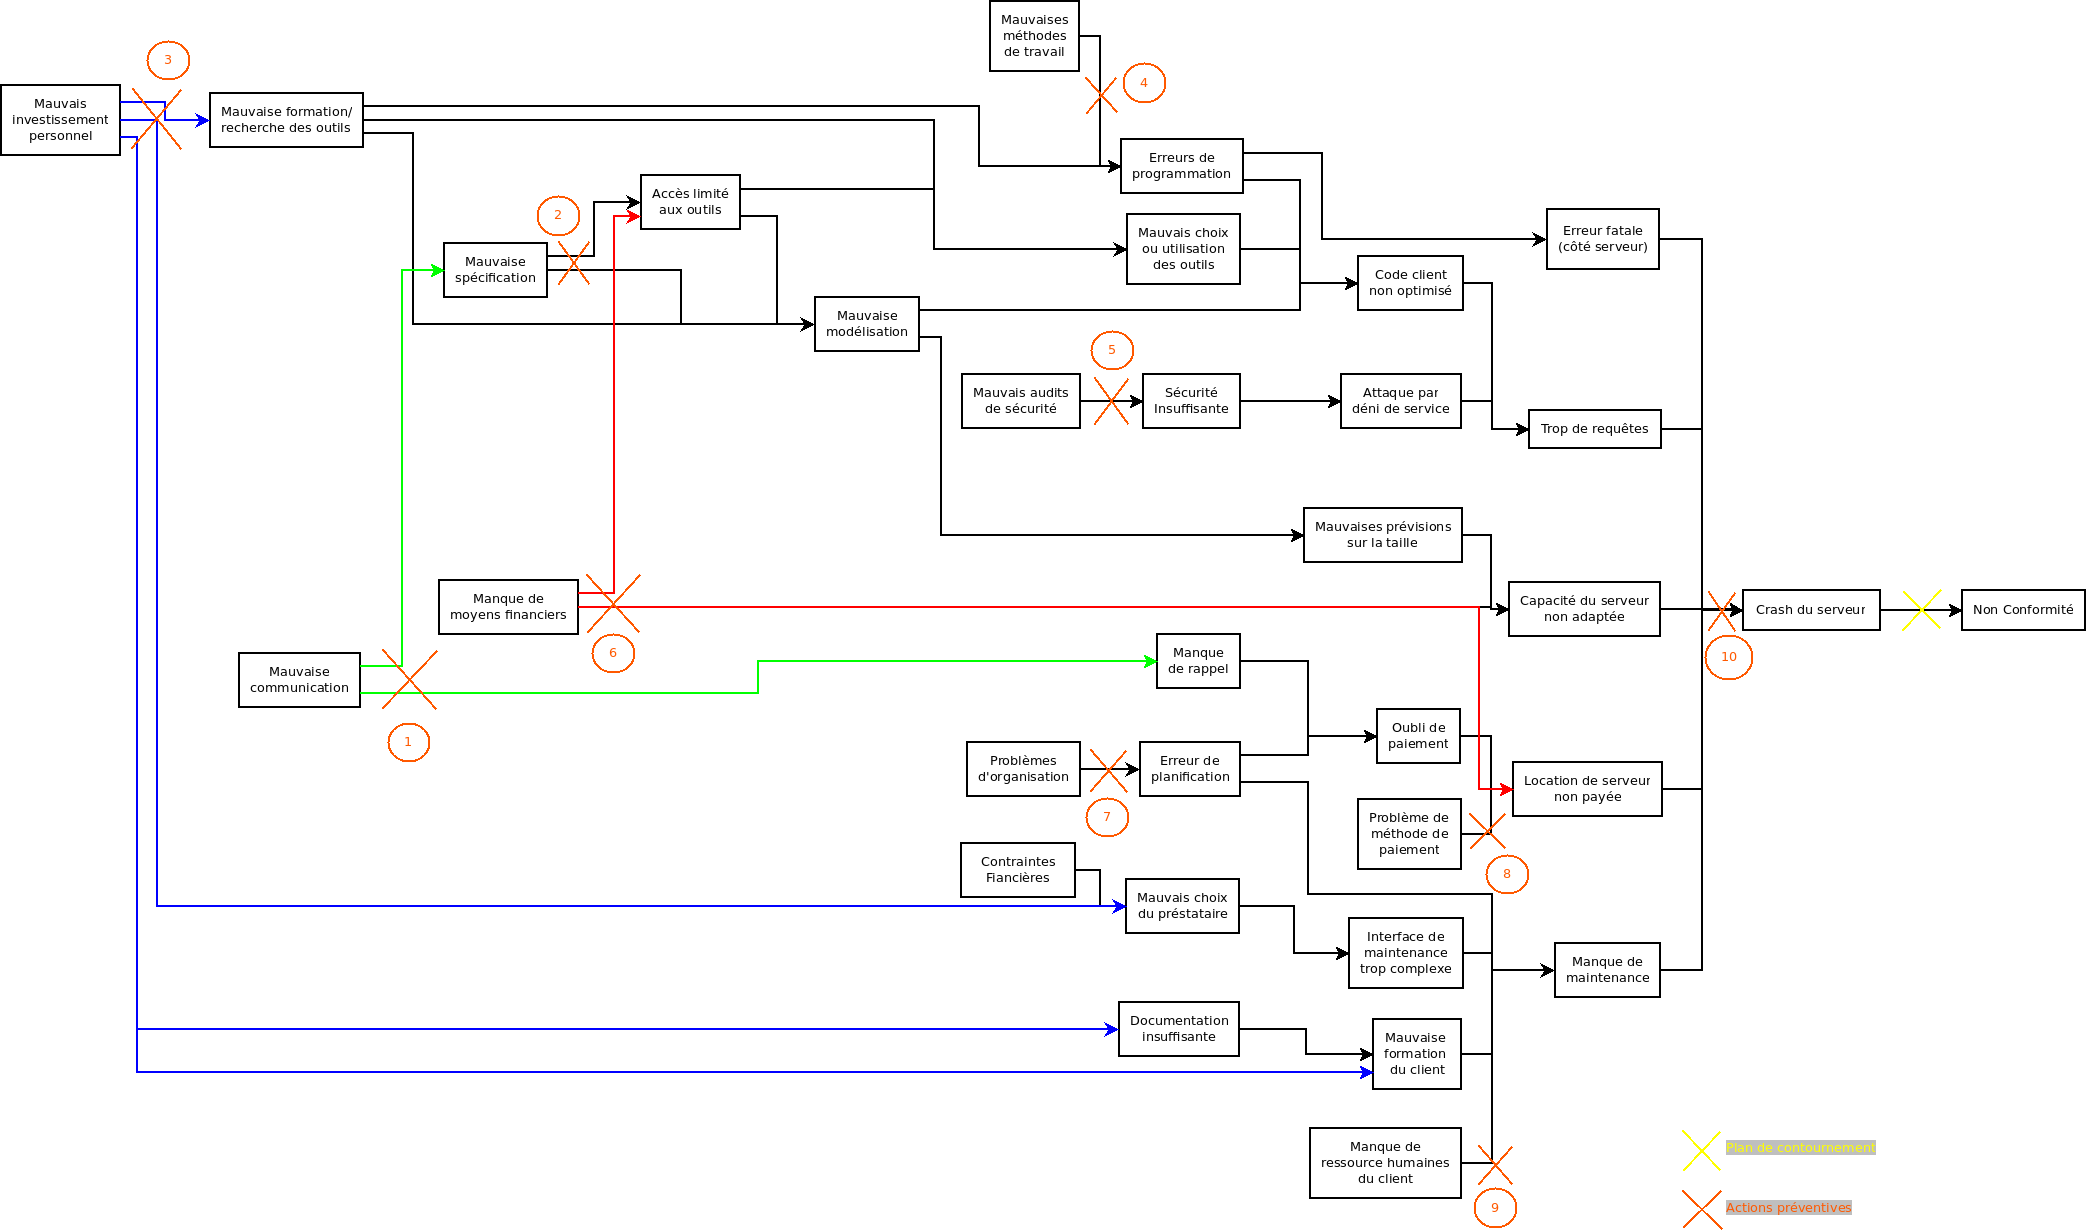
\includegraphics[scale=0.35]{images/AnalyseRisque_nPourquoi.png}
\end{figure}
\end{landscape}
\chapter*{Fiche de Risque 002}
\section*{Informations générales}

\begin{table}[H]
\centering
	\begin{tabularx}{16.8cm}{|X|X|}
	\hline
	\rowcolor{gray!40} Numéro du risque & Type du risque \\
	\hline
	002 & Mauvaise ambiance dans l'équipe / problème de cohésion \\
	\hline
	\end{tabularx}
\end{table}

\begin{table}[H]
\centering
	\begin{tabularx}{16.8cm}{|X|X|X|}
	\hline
	\rowcolor{gray!40} Date & Visa du \RQ & Visa du \CP \\
	\hline
	 28/01/16 & pgpic & pgpic \\
	\hline
	\end{tabularx}
\end{table}

\begin{table}[H]
\centering
	\begin{tabularx}{16.8cm}{|X|X|X|X|}
	\hline
	\rowcolor{gray!40} Pilote & Activité WBS & Compte WBS & Phase d'apparition \\
	\hline
	 \Michel & Suivre les Risques et Opportunités & 1.2.3.2 & À partir du début du projet\\
	\hline
	\end{tabularx}
\end{table}

\section*{Description du risque}

\subsection*{Résumé}
	Le risque lié à la mauvaise ambiance dans le \PICCourt{} ou au problème de cohésion  peut entraîner une mauvaise façon de travailler et donc influencer la qualité du produit finale.
	
\subsection*{Analyse des causes}
	voir figure.

\subsection*{Criticité}

\begin{table}[H]
\centering
	\begin{tabularx}{16.8cm}{|>{\columncolor{gray!40}}X|X|}
	\hline
	Gravité & 3\\
	\hline
	Probabilité & 2\\
	\hline
	Criticité & A surveiller\\
	\hline
	\end{tabularx}
\end{table}
\newpage

\section*{Actions}
\subsection*{Actions préventives}

%\begin{table}[H]
\centering
	\begin{longtable}{|p{7cm}|p{7cm}|}
	\hline
	\rowcolor{gray!40} Numéro de cause & Actions préventives \\
	\hline
	 1 & \begin{itemize}
	 	\item Mettre en place des Team Building
	 	\item L'équipe établit des règles communes de fonctionnement des \PICCourt{}
	 	\item Le chef projet met en place des règles de communication de type DESC
	 \end{itemize} \\
	\hline
	2 & \begin{itemize}
		\item Entraide de l'équipe
		\item Partage du travail
	\end{itemize}	 \\
	\hline
	3 & \begin{itemize}
		\item Soutien moral
	\end{itemize} \\
	\hline
	
	\end{longtable}
%\end{table}

\flushleft
\subsection*{Plan de contournement}

\begin{enumerate}
	\item Le chef de projet identifie l'objet du conflit et interroge chaque membre concerné.
	\item Le chef de projet prend le rôle de médiateur et convoque les membres concernés à une réunion de négociation puis leur demande de mettre en oeuvre la méthode DESC.
\end{enumerate}

\section*{Décision de clôture}
Par le \CP{} et le pilote du risque.
\begin{table}[H]
\centering
	\begin{tabularx}{16.8cm}{|X|X|}
	\hline
	\rowcolor{gray!40} Date de clôture & Raison de la clôture \\
	\hline
	  & \\
	\hline
	\end{tabularx}
\end{table}

\section*{Historique des modifications}
\begin{table}[H]
\centering
	\begin{tabularx}{16.8cm}{|X|X|}
	\hline
	Date & Modification \\
	\hline
	  & \\
	\hline
	\end{tabularx}
\end{table}
\newpage

\begin{landscape}
\begin{figure}
	\centering
	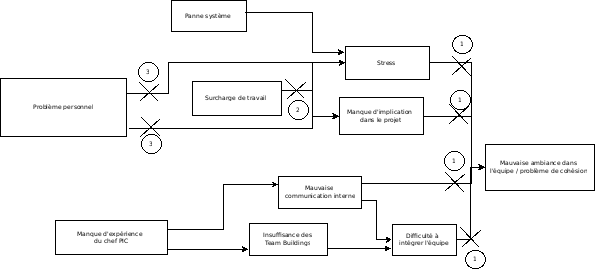
\includegraphics[scale=0.84]{images/AnalyseRisque_nPourquoi_FDR002}
\end{figure}
\end{landscape}
\chapter*{Fiche de Risque 003}
% version 1.00	date 29/01/2016  	Auteur Pierre Porche

\section*{Informations générales}
 
\begin{table}[h]
\centering
	\begin{tabularx}{16.8cm}{|X|X|}
	\hline
	\rowcolor{gray!40} Numéro du risque & Type du risque \\
	\hline
	003 & Absence collective \\
	\hline
	\end{tabularx}
\end{table}

\begin{table}[h]
\centering
	\begin{tabularx}{16.8cm}{|X|X|X|}
	\hline
	\rowcolor{gray!40} Date & Visa du \RQ & Visa du \CP \\
	\hline
	 27/01/16 & pgpic & pgpic \\
	\hline
	\end{tabularx}
\end{table}

\begin{table}[h]
\centering
	\begin{tabularx}{16.8cm}{|X|X|X|X|}
	\hline
	\rowcolor{gray!40} Pilote & Activité WBS & Compte WBS & Phase d'apparition \\
	\hline
	 \Pierre & Suivre les Risques et Opportunités & 1.2.3.2 & À partir du début du projet \\
	\hline
	\end{tabularx}
\end{table}

\section*{Description du risque}

\subsection*{Résumé}
	Le risque lié à une absence collective peut entraîner un ralentissement voire un arrêt total du travail et donc perturber grandement le planning.
	
\subsection*{Analyse des causes}
	voir figure \ref{risque absence collective}.

\subsection*{Criticité}

\begin{table}[h]
\centering
	\begin{tabularx}{12.8cm}{|>{}X|X|}
	\hline
	Gravité & 4\\
	\hline
	Probabilité & 1\\
	\hline
	Criticité & Critique\\
	\hline
	\end{tabularx}
\end{table}
\newpage

\section*{Actions}
\subsection*{Actions préventives}

%\begin{table}[H]
\centering
	\begin{longtable}{|p{7cm}|p{7cm}|}
	\hline
	\rowcolor{gray!40} Numéro de cause & Actions préventives \\
	\hline
	 1 & \begin{itemize}
	 	\item Prévenir en cas de maladie
	 	\item Le \CP{} doit se tenir au courant des épidémies en temps réel
	 \end{itemize} \\

	\hline
	2 & \begin{itemize}
		\item Avoir une bonne planification
	\end{itemize} \\
	\hline
	3 & \begin{itemize}
		\item Se tenir au courant des faits d'actualité
	\end{itemize} \\
	\hline
	\end{longtable}
%\end{table}

\flushleft
\subsection*{Plan de contournement}

\begin{enumerate}
	\item Résumer l'état des présences de chacun.
	\item Prévenir le client ainsi que le tuteur pédagogique.
	\item Réorganiser le planning de manière à avoir une perte de productivité la moins importante possible.
	\item Réorganiser le planning de nouveau dès le retour des absents.
\end{enumerate}

\section*{Décision de clôture}
Par le \CP{} et le pilote du risque.
\begin{table}[H]
\centering
	\begin{tabularx}{12.8cm}{|X|X|}
	\hline
	\rowcolor{gray!40} Date de clôture & Raison de la clôture \\
	\hline
	  & \\
	\hline
	\end{tabularx}
\end{table}

\section*{Historique des modifications}
\begin{table}[H]
\centering
	\begin{tabularx}{12.8cm}{|X|X|}
	\hline
	\rowcolor{gray!40} Date & Modification \\
	\hline
	  & \\
	\hline
	\end{tabularx}
\end{table}
\newpage


\begin{figure}
	\centering
	\includegraphics[scale=0.2]{images/nPourquoiFDR003}
        \caption{\label{risque absence collective}risque absence collective - méthode des n pourquoi}
\end{figure}

\chapter*{Fiche de Risque 004}
% version 1.02	date 20/04/2016  	Auteur Pierre Porche
% version 1.01	date 29/03/2016  	Auteur Pierre Porche
% version 1.00	date 29/01/2016  	Auteur Julie Pain

\section*{Informations générales}
 
\begin{table}[H]
\centering
	\begin{tabularx}{16.8cm}{|X|X|}
	\hline
	\rowcolor{gray!40} Numéro du risque & Type du risque \\
	\hline
	004 & Mauvaise communication avec le client \\
	\hline
	\end{tabularx}
\end{table}

\begin{table}[H]
\centering
	\begin{tabularx}{16.8cm}{|X|X|X|}
	\hline
	\rowcolor{gray!40} Date & Visa du \RQ & Visa du \CP \\
	\hline
	 29/01/2016 & pgpic & pgpic \\
	\hline
	\end{tabularx}
\end{table}

\begin{table}[H]
\centering
	\begin{tabularx}{16.8cm}{|X|X|X|X|}
	\hline
	\rowcolor{gray!40} Pilote & Activité WBS & Compte WBS & Phase d'apparition \\
	\hline
	 \Julie & Suivre les Risques et Opportunités & 1.2.3.2 & À partir du début du projet\\
	\hline
	\end{tabularx}
\end{table}

\section*{Description du risque}

\subsection*{Résumé}
	Une mauvaise communication ou une absence de communication avec le client peut entraîner une mauvaise compréhension des besoins du client. Cela peut avoir des conséquences sur la réalisation du produit, notamment une insatisfaction du client ou un rendu en retard du produit. \\
	La mauvaise communication peut être dûe à la lenteur ou à l'absence de réponse du client aux mails du \CP{} ou à un défaut ou retard d'envoi des mails au client.
\subsection*{Analyse des causes}
	voir figure \ref{risque mauvaise communication client}.

\subsection*{Criticité}

\begin{table}[H]
\centering
	\begin{tabularx}{16.8cm}{|>{\columncolor{gray!40}}X|X|}
	\hline
	Gravité & 3\\
	\hline
	Probabilité & 3\\
	\hline
	Criticité & Critique \\
	\hline
	\end{tabularx}
\end{table}
\newpage

\section*{Actions}
\subsection*{Actions préventives}

\centering
	\begin{longtable}{|p{7cm}|p{7cm}|}
	\hline
	\rowcolor{gray!40} Numéro de cause & Actions préventives \\
	\hline
	1 & \begin{itemize}
		\item Mettre en place un planning.
		\end{itemize} \\
	\hline
	2 & \begin{itemize}
		\item Faire valider les \CRC{} par le client.
		\end{itemize} \\
	\hline
	3 & \begin{itemize}
		\item Répondre aux mails du client le plus tôt possible.
		\end{itemize} \\
	\hline
	4 & \begin{itemize}
		\item Définir des règles de communication.
	\end{itemize} \\
	\hline
	5 & \begin{itemize}
		\item Réaliser des actions de Team Building.
	\end{itemize} \\
	\hline
	6 & \begin{itemize}
		\item Réaliser des tutorats communication.
	\end{itemize} \\
	\hline
	\end{longtable}

\flushleft
\subsection*{Plan de contournement}

\begin{enumerate}
	\item Récupérer la version du document la plus récente possible.
	\item Ré-imprimer le document et le refaire valider si besoin.
	\item Refaire le travail perdu le plus vite possible.
\end{enumerate}

\section*{Décision de clôture}
Par le \CP{} et le pilote du risque.
\begin{table}[H]
\centering
	\begin{tabularx}{16.8cm}{|X|X|}
	\hline
	\rowcolor{gray!40} Date de clôture & Raison de la clôture \\
	\hline
	  & \\
	\hline
	\end{tabularx}
\end{table}

\section*{Historique des modifications}
\begin{table}[H]
\centering
	\begin{tabularx}{16.8cm}{|X|X|}
	\hline	
        \rowcolor{gray!40} Date & Modification \\
        
        \hline
	29/03/2016 & modification de la probabilité de 2 à 3 pour cause de vacances du client. \\
	\hline
	23/03/2016 & modification de la probabilité de 1 à 2 pour cause de vacances du client. \\
	\hline
	14/03/2016 & modification de la probabilité\\
	\hline
	\end{tabularx}
\end{table}
\newpage

\begin{figure}
	\centering
	\includegraphics[scale=0.8]{images/nPourquoiFDR004}
	\caption{\label{risque mauvaise communication client}risque mauvaise communication client - méthode des n pourquoi}
\end{figure}

\chapter*{Fiche de Risque 005}
\section*{Informations générales}
 
\begin{table}[H]
\centering
	\begin{tabularx}{16.8cm}{|X|X|}
	\hline
	\rowcolor{gray!40} Numéro du risque & Type du risque \\
	\hline
	005 & Mauvaise plannification \\
	\hline
	\end{tabularx}
\end{table}

\begin{table}[H]
\centering
	\begin{tabularx}{16.8cm}{|X|X|X|}
	\hline
	\rowcolor{gray!40} Date & Visa du \RQ & Visa du \CP \\
	\hline
	 28/01/2016 & pgpic & pgpic \\
	\hline
	\end{tabularx}
\end{table}

\begin{table}[H]
\centering
	\begin{tabularx}{16.8cm}{|X|X|X|X|}
	\hline
	\rowcolor{gray!40} Pilote & Activité WBS & Compte WBS & Phase d'apparition \\
	\hline
	 \Florian & Suivre les Risques et Opportunités & 1.2.3.2 & À partir du début du projet\\
	\hline
	\end{tabularx}
\end{table}

\section*{Description du risque}

\subsection*{Résumé}
	La mauvaise planification concerne principalement l’appréciation des délais des tâches et peut être expliquée par l’inexpérience du Chef PIC. Elle peut entrainer des retards de livraison des lots.

\subsection*{Analyse des causes}
	voir figure \ref{risque perte de document}.

\subsection*{Criticité}

\begin{table}[H]
\centering
	\begin{tabularx}{16.8cm}{|>{\columncolor{gray!40}}X|X|}
	\hline
	Gravité & 3\\
	\hline
	Probabilité & 2\\
	\hline
	Criticité & A surveiller\\
	\hline
	\end{tabularx}
\end{table}
\newpage

\section*{Actions}
\subsection*{Actions préventives}

\centering
	\begin{longtable}{|p{7cm}|p{7cm}|}
	\hline
	\rowcolor{gray!40} Numéro de cause & Actions préventives \\
	\hline
	1 & \begin{itemize}
		\item Formation au logiciel PGPIC.
                \item Mise en place de mêlées quotidiennes.
		\end{itemize} \\
	\hline
	2 & \begin{itemize}
		\item Le \CPACourt{} doit se tenir au courant des actions du CPCourt{}.
		\end{itemize} \\
	\hline
	\end{longtable}

\section*{Décision de clôture}
Par le \CP{} et le pilote du risque.
\begin{table}[H]
\centering
	\begin{tabularx}{16.8cm}{|X|X|}
	\hline
	\rowcolor{gray!40} Date de clôture & Raison de la clôture \\
	\hline
	  & \\
	\hline
	\end{tabularx}
\end{table}

\section*{Historique des modifications}
\begin{table}[H]
\centering
	\begin{tabularx}{16.8cm}{|X|X|}
	\hline
	Date & Modification \\
	\hline
	  & \\
	\hline
	\end{tabularx}
\end{table}
\newpage

\begin{landscape}
\begin{figure}
	\centering
	\includegraphics[scale=0.35]{images/AnalyseRisque_nPourquoi_FDR005}
	\caption{\label{risque perte de document}risque mauvaise plannification - méthode des n pourquoi}
\end{figure}
\end{landscape}

\chapter*{Fiche de Risque 006}
\section*{Informations générales}

\begin{table}[H]
\centering
	\begin{tabularx}{16.8cm}{|X|X|}
	\hline
	\rowcolor{gray!40} Numéro du risque & Type du risque \\
	\hline
	006 & Mauvaise mise en route du second semestre \\
	\hline
	\end{tabularx}
\end{table}

\begin{table}[H]
\centering
	\begin{tabularx}{16.8cm}{|X|X|X|}
	\hline
	\rowcolor{gray!40} Date & Visa du \RQ & Visa du \CP \\
	\hline
	 29/01/16 & pgpic & pgpic \\
	\hline
	\end{tabularx}
\end{table}

\begin{table}[H]
\centering
	\begin{tabularx}{16.8cm}{|X|X|X|X|}
	\hline
	\rowcolor{gray!40} Pilote & Activité WBS & Compte WBS & Phase d'apparition \\
	\hline
	 \Melissa & Suivre les Risques et Opportunités & 1.2.3.2 & À partir du début de la deuxième période. \\
	\hline
	\end{tabularx}
\end{table}

\section*{Description du risque}

\subsection*{Résumé}
	Le risque lié à la mauvaise mise en route du second semestre peut entraîner une mauvaise façon de travailler et donc influencer la qualité du produit finale.
	
\subsection*{Analyse des causes}
	voir figure.

\subsection*{Criticité}

\begin{table}[H]
\centering
	\begin{tabularx}{16.8cm}{|>{\columncolor{gray!40}}X|X|}
	\hline
	Gravité & 3\\
	\hline
	Probabilité & 3\\
	\hline
	Criticité & Critique\\
	\hline
	\end{tabularx}
\end{table}
\newpage

\section*{Actions}
\subsection*{Actions préventives}

%\begin{table}[H]
\centering
	\begin{longtable}{|p{7cm}|p{7cm}|}
	\hline
	\rowcolor{gray!40} Numéro de cause & Actions préventives \\
	\hline
	 1 & \begin{itemize}
	 	\item Mettre en place des outils de connaissance tels que des fiches. 
	 	\item Bien définir les rôles 
	 \end{itemize} \\
	\hline
	2 & \begin{itemize}
		\item Vérification du travail par le le \RD
	\end{itemize}	 \\
	\hline
	3 & \begin{itemize}
		\item Vérification des diagrammes PERT et GANT par le \CPA
	\end{itemize} \\
	\hline
	4 & \begin{itemize}
		\item Former le \CPA et \RQA en vue de la passation de pouvoir de la première à la seconde période. 
	\end{itemize} \\
	\hline
	
	\end{longtable}
%\end{table}

\flushleft
\subsection*{Plan de contournement}

\begin{enumerate}
	\item Contacter les anciens \CP et \RQ et leur demander des conseils 
\end{enumerate}

\section*{Décision de clôture}
Par le \CP{} et le pilote du risque.
\begin{table}[H]
\centering
	\begin{tabularx}{16.8cm}{|X|X|}
	\hline
	\rowcolor{gray!40} Date de clôture & Raison de la clôture \\
	\hline
	  & \\
	\hline
	\end{tabularx}
\end{table}

\section*{Historique des modifications}
\begin{table}[H]
\centering
	\begin{tabularx}{16.8cm}{|X|X|}
	\hline
	Date & Modification \\
	\hline
	  & \\
	\hline
	\end{tabularx}
\end{table}
\newpage

\begin{landscape}
\begin{figure}
	\centering
	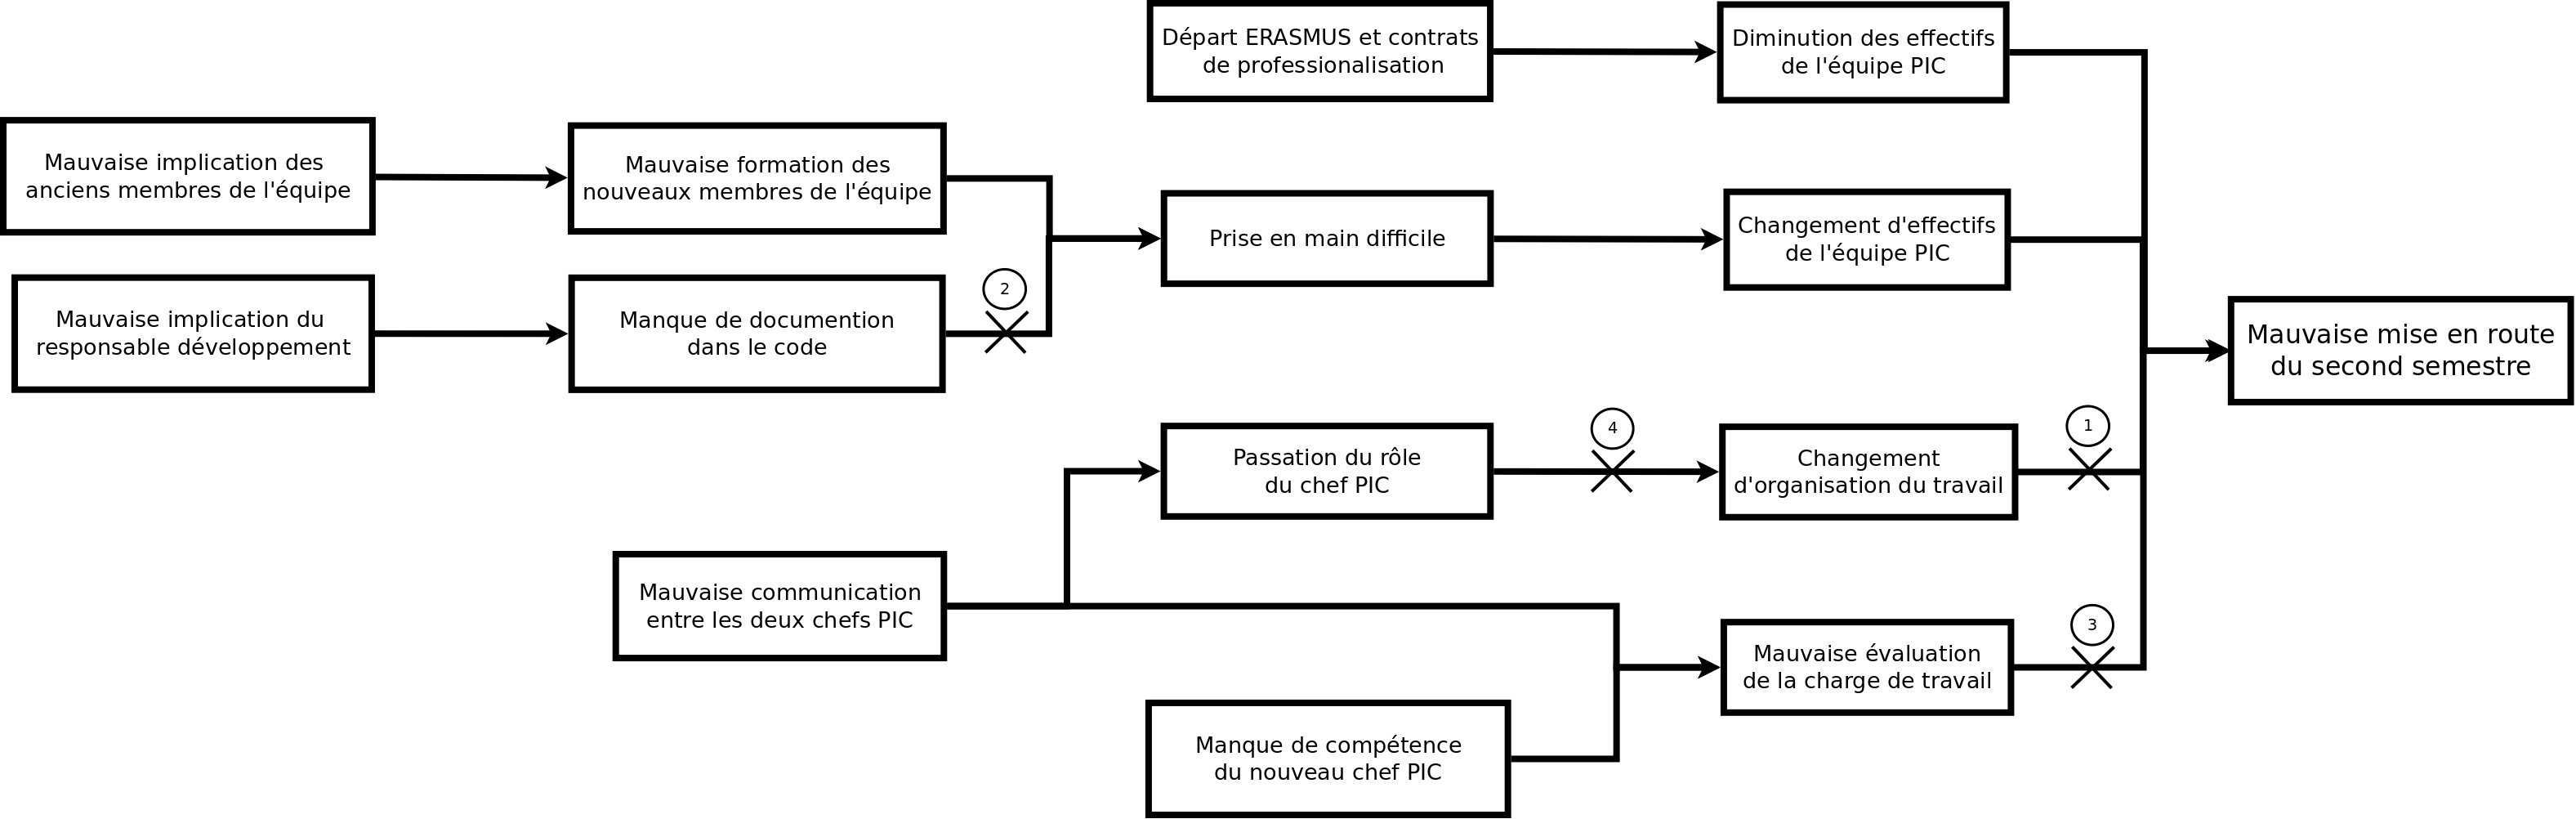
\includegraphics[scale=1.5]{images/AnalyseRisque_nPourquoi_FDR006}
\end{figure}
\end{landscape}
\chapter*{Fiche de Risque 007}
% version 1.00	date 29/01/2016  	Auteur Mathieu Médici

\section*{Informations générales}
 
\begin{table}[H]
\centering
	\begin{tabularx}{16.8cm}{|X|X|}
	\hline
	\rowcolor{gray!40} Numéro du risque & Type du risque \\
	\hline
	007 & Perte de documents \\
	\hline
	\end{tabularx}
\end{table}

\begin{table}[H]
\centering
	\begin{tabularx}{16.8cm}{|X|X|X|}
	\hline
	\rowcolor{gray!40} Date & Visa du \RQ & Visa du \CP \\
	\hline
	 28/01/2016 & pgpic & pgpic \\
	\hline
	\end{tabularx}
\end{table}

\begin{table}[H]
\centering
	\begin{tabularx}{16.8cm}{|X|X|X|X|}
	\hline
	\rowcolor{gray!40} Pilote & Activité WBS & Compte WBS & Phase d'apparition \\
	\hline
	 \Melissa & Suivre les Risques et Opportunités & 1.2.3.2 & À partir du début du projet\\
	\hline
	\end{tabularx}
\end{table}

\section*{Description du risque}

\subsection*{Résumé}
	Le risque lié à la perte de documents peut entrainer une perte du travail réalisé et donc une perte de temps sur l'avancement du projet.
	
\subsection*{Analyse des causes}
	voir figure \ref{risque perte de document}.

\subsection*{Criticité}

\begin{table}[H]
\centering
	\begin{tabularx}{16.8cm}{|>{\columncolor{gray!40}}X|X|}
	\hline
	Gravité & 4\\
	\hline
	Probabilité & 1\\
	\hline
	Criticité & Critique\\
	\hline
	\end{tabularx}
\end{table}
\newpage

\section*{Actions}
\subsection*{Actions préventives}

\centering
	\begin{longtable}{|p{7cm}|p{7cm}|}
	\hline
	\rowcolor{gray!40} Numéro de cause & Actions préventives \\
	\hline
	1 & \begin{itemize}
		\item Formation des membres de l'équipe aux outils
		\end{itemize} \\
	\hline
	2 & \begin{itemize}
		\item Vérification du travail du \RGC{} par le \CP
		\item Vérification du nommage et de l'archivage par le \RGC{} toutes les semaines
		\end{itemize} \\
	\hline
	3 & \begin{itemize}
		\item Formation du \RGC
		\end{itemize} \\
	\hline
	4 & \begin{itemize}
		\item Faire un clone de l'archive toutes les semaines
	\end{itemize} \\
	\hline
	\end{longtable}

\flushleft
\subsection*{Plan de contournement}

\begin{enumerate}
	\item Récupérer la version du document la plus récente possible
	\item Ré-imprimer le document et le refaire valider si besoin
	\item Refaire le travail perdu le plus vite possible
\end{enumerate}

\section*{Décision de clôture}
Par le \CP{} et le pilote du risque.
\begin{table}[H]
\centering
	\begin{tabularx}{16.8cm}{|X|X|}
	\hline
	\rowcolor{gray!40} Date de clôture & Raison de la clôture \\
	\hline
	  & \\
	\hline
	\end{tabularx}
\end{table}

\section*{Historique des modifications}
\begin{table}[H]
\centering
	\begin{tabularx}{16.8cm}{|X|X|}
	\hline
	\rowcolor{gray!40} Date & Modification \\
	\hline
	 06/09/2016 & modification pilote car changement d'équipe \\
	\hline
	\end{tabularx}
\end{table}
\newpage

\begin{figure}
	\centering
	\includegraphics[scale=0.75]{images/nPourquoiFDR007}
	\caption{\label{risque perte de document}risque perte de document - méthode des n pourquoi}
\end{figure}

\chapter*{Fiche de Risque 008}
% version 1.00	date 29/01/2016  	Auteur Julie Pain

\section*{Informations générales}
 
\begin{table}[H]
\centering
	\begin{tabularx}{16.8cm}{|X|X|}
	\hline
	\rowcolor{gray!40} Numéro du risque & Type du risque \\
	\hline
	008 & Indisposition du client pour le passage d'une recette \\
	\hline
	\end{tabularx}
\end{table}

\begin{table}[H]
\centering
	\begin{tabularx}{16.8cm}{|X|X|X|}
	\hline
	\rowcolor{gray!40} Date & Visa du \RQ & Visa du \CP \\
	\hline
	 29/01/2016 & pgpic & pgpic \\
	\hline
	\end{tabularx}
\end{table}

\begin{table}[H]
\centering
	\begin{tabularx}{16.8cm}{|X|X|X|X|}
	\hline
	\rowcolor{gray!40} Pilote & Activité WBS & Compte WBS & Phase d'apparition \\
	\hline
	 \Julie & Suivre les Risques et Opportunités & 1.2.3.2 & À partir du début du projet\\
	\hline
	\end{tabularx}
\end{table}

\section*{Description du risque}

\subsection*{Résumé}
	Une indisponibilité du client lors d'un rendez-vous prévu pour un passage de recette peut retarder la livraison du produit par l'équipe. 
	
\subsection*{Analyse des causes}
	voir figure \ref{risque indisposition client}.

\subsection*{Criticité}

\begin{table}[H]
\centering
	\begin{tabularx}{16.8cm}{|>{\columncolor{gray!40}}X|X|}
	\hline
	Gravité & 3\\
	\hline
	Probabilité & 3\\
	\hline
	Criticité & \`A surveiller\\
	\hline
	\end{tabularx}
\end{table}
\newpage

\section*{Actions}
\subsection*{Actions préventives}

\centering
	\begin{longtable}{|p{7cm}|p{7cm}|}
	\hline
	\rowcolor{gray!40} Numéro de cause & Actions préventives \\
	\hline
	1 & \begin{itemize}
		\item Rappel des rendez-vous quelques jours avant
		\end{itemize} \\
	\hline
	2 & \begin{itemize}
		\item Prévoir un deuxième créneau de rendez-vous
		\end{itemize} \\
	\hline
	3 & \begin{itemize}
		\item Vérification de la planification \CP{} par le \CPA{}
		\end{itemize} \\
	\hline
	\end{longtable}

\flushleft
\subsection*{Plan de contournement}

\begin{enumerate}
	\item Fixer une nouvelle date de recette avec le client dans les meilleurs délais.
\end{enumerate}

\section*{Décision de clôture}
Par le \CP{} et le pilote du risque.
\begin{table}[H]
\centering
	\begin{tabularx}{16.8cm}{|X|X|}
	\hline
	\rowcolor{gray!40} Date de clôture & Raison de la clôture \\
	\hline
	  & \\
	\hline
	\end{tabularx}
\end{table}

\section*{Historique des modifications}
\begin{table}[H]
\centering
	\begin{tabularx}{16.8cm}{|X|X|}
	\hline
	\rowcolor{gray!40} Date & Modification \\
	\hline
	  & \\
	\hline
	\end{tabularx}
\end{table}
\newpage


\begin{figure}
	\centering
	\includegraphics[scale=1.2]{images/nPourquoiFDR008}
	\caption{\label{risque indisposition client}risque indisposition du client pour le passage d'une recette - méthode des n pourquoi}
\end{figure}

\chapter*{Fiche de Risque 009}
% version 1.01	date 14/03/2016  	Auteur Matthieu Martins-Baltar Pierre Porche

\section*{Informations générales}
 
\begin{table}[H]
\centering
	\begin{tabularx}{16.8cm}{|X|X|}
	\hline
	\rowcolor{gray!40} Numéro du risque & Type du risque \\
	\hline
	009 & Absence de serveur extérieur \\
	\hline
	\end{tabularx}
\end{table}

\begin{table}[H]
\centering
	\begin{tabularx}{16.8cm}{|X|X|X|}
	\hline
	\rowcolor{gray!40} Date & Visa du \RQ & Visa du \CP \\
	\hline
	 28/01/2016 & pgpic & pgpic \\
	\hline
	\end{tabularx}
\end{table}

\begin{table}[H]
\centering
	\begin{tabularx}{16.8cm}{|X|X|X|X|}
	\hline
	\rowcolor{gray!40} Pilote & Activité WBS & Compte WBS & Phase d'apparition \\
	\hline
	 \Matthieu & Suivre les Risques et Opportunités & 1.2.3.2 & À partir du début du projet\\
	\hline
	\end{tabularx}
\end{table}

\section*{Description du risque}

\subsection*{Résumé}
	Le risque lié à l'absence de serveur gratuit pour déployer notre livrable nous obligerait à nous retourner vers une solution payante qui ne satisferait pas le client.
	
\subsection*{Analyse des causes}
	voir figure \ref{risque pas de serveur ext}.

\subsection*{Criticité}

\begin{table}[H]
\centering
	\begin{tabularx}{16.8cm}{|>{\columncolor{gray!40}}X|X|}
	\hline
	Gravité & 4\\
	\hline
	Probabilité & 2\\
	\hline
	Criticité & Critique\\
	\hline
	\end{tabularx}
\end{table}
\newpage

\section*{Actions}
\subsection*{Actions préventives}

\centering
	\begin{longtable}{|p{7cm}|p{7cm}|}
	\hline
	\rowcolor{gray!40} Numéro de cause & Actions préventives \\
	\hline
	1 & \begin{itemize}
		\item Faire une bonne recherche des hébergeurs susceptibles de fournir un serveur
		\end{itemize} \\
	\hline
	2 & \begin{itemize}
		\item Formation des membres de l'équipe aux démarches de mécénat
		\end{itemize} \\
	\hline
	3 & \begin{itemize}
		\item Trouver une solution gratuite
		\end{itemize} \\
	\hline
	4 & \begin{itemize}
		\item Se rabattre sur une solution payante avec accord du client
	\end{itemize} \\
	\hline
	5 & \begin{itemize}
		\item Si une solution parmi INSA, hébergeur privé ou Unicef France est impossible, se rabattre sur l'une des deux autres solutions.
	\end{itemize} \\
	\hline
	6 & \begin{itemize}
		\item Former le \CP{} à la planification
		\item Bien prévoir les temps nécessaires à chaque tâche
		\end{itemize} \\
	\hline
	7 & \begin{itemize}
		\item Avoir une méthode de paiement de secours
		\item Se renseigner auprès des prestataires
		\item Demander au département les méthodes de paiement autorisées
		\end{itemize} \\
	\hline
	\end{longtable}

\flushleft
\subsection*{Plan de contournement}

\begin{enumerate}
	\item Faire une demande spéciale auprès de l'INSA pour obtenir un serveur en urgence.
\end{enumerate}

%\begin{enumerate}
%	\item Faire accepter au client d'avoir recours à une solution payante
%
%	\item Rechercher et comparer les offres des différents prestataires.
%
%	\item Sélectionner une offre de serveur à un prix raisonnable
%
%	\item Confirmer auprès du client que l'offre et le prix sont acceptables
%
%	\item Utiliser ce serveur en remplacement à une solution gratuite
%\end{enumerate}

\section*{Décision de clôture}
Par le \CP{} et le pilote du risque.
\begin{table}[H]
\centering
	\begin{tabularx}{16.8cm}{|X|X|}
	\hline
	\rowcolor{gray!40} Date de clôture & Raison de la clôture \\
	\hline
	  & \\
	\hline
	\end{tabularx}
\end{table}

\section*{Historique des modifications}
\begin{table}[H]
\centering
	\begin{tabularx}{16.8cm}{|X|X|}
	\hline
	\rowcolor{gray!40} Date & Modification \\
	\hline
	 19/10/2016 & probabilité diminuée dû à un récent contact avec Quantic Télecom \\
	\hline
	 27/04/2016 & probabilité modifiée car la date approche \\
	\hline
	 14/03/2016 & modification probabilité \\
	\hline
	\end{tabularx}
\end{table}
\newpage

\begin{figure}
	\centering
	\includegraphics[scale=0.15]{images/nPourquoiFDR009}
	\caption{\label{risque pas de serveur ext}risque pas de serveur extérieur - méthode des n pourquoi}
\end{figure}

\chapter*{Fiche de Risque 010}
% version 1.00	date 29/01/2016  	Auteur Pierre Porche

\section*{Informations générales}
 
\begin{table}[h]
\centering
	\begin{tabularx}{16.8cm}{|X|X|}
	\hline
	\rowcolor{gray!40} Numéro du risque & Type du risque \\
	\hline
	010 & Problème avec la CNIL\\
	\hline
	\end{tabularx}
\end{table}

\begin{table}[h]
\centering
	\begin{tabularx}{12.8cm}{|X|X|X|}
	\hline
	\rowcolor{gray!40} Date & Visa du \RQ & Visa du \CP \\
	\hline
	 27/01/16 & pgpic & pgpic \\
	\hline
	\end{tabularx}
\end{table}

\begin{table}[h]
\centering
	\begin{tabularx}{12.8cm}{|X|X|X|X|}
	\hline
	\rowcolor{gray!40} Pilote & Activité WBS & Compte WBS & Phase d'apparition \\
	\hline
	 \Pierre & Suivre les Risques et Opportunités & 1.2.3.2 & À partir du remplissage de la BD \\
	\hline
	\end{tabularx}
\end{table}

\section*{Description du risque}

\subsection*{Résumé}
	Le risque lié à un problème avec la CNIL peut entraîner des problèmes d'ordre juridique pouvant stopper brutalement le projet.
	
\subsection*{Analyse des causes}
	voir figure \ref{risque pb cnil}.

\subsection*{Criticité}

\begin{table}[h]
\centering
	\begin{tabularx}{12.8cm}{|>{}X|X|}
	\hline
	Gravité & 3\\
	\hline
	Probabilité & 2\\
	\hline
	Criticité & A surveiller\\
	\hline
	\end{tabularx}
\end{table}
\newpage

\section*{Actions}
\subsection*{Actions préventives}

%\begin{table}[H]
\centering
	\begin{longtable}{|p{7cm}|p{7cm}|}
	\hline
	\rowcolor{gray!40} Numéro de cause & Actions préventives \\
	\hline
	 1 & \begin{itemize}
	 	\item S'informer sur la législation en vigueur.
	 \end{itemize} \\
	\hline

	\end{longtable}
%\end{table}

\flushleft
\subsection*{Plan de contournement}

\begin{enumerate}
	\item Déterminer les cause de l'alerte de la CNIL
	\item Prévenir le client ainsi que le tuteur pédagogique
	\item Revoir notre gestion des informations personnelles
	\item Élaborer un nouveau dossier pour la CNIL
\end{enumerate}

\section*{Décision de clôture}
Par le \CP{} et le pilote du risque.
\begin{table}[H]
\centering
	\begin{tabularx}{12.8cm}{|X|X|}
	\hline
	\rowcolor{gray!40} Date de clôture & Raison de la clôture \\
	\hline
	  & \\
	\hline
	\end{tabularx}
\end{table}

\section*{Historique des modifications}
\begin{table}[H]
\centering
	\begin{tabularx}{12.8cm}{|X|X|}
	\hline
	\rowcolor{gray!40} Date & Modification \\
	\hline
	  & \\
	\hline
	\end{tabularx}
\end{table}
\newpage


\begin{figure}
	\centering
	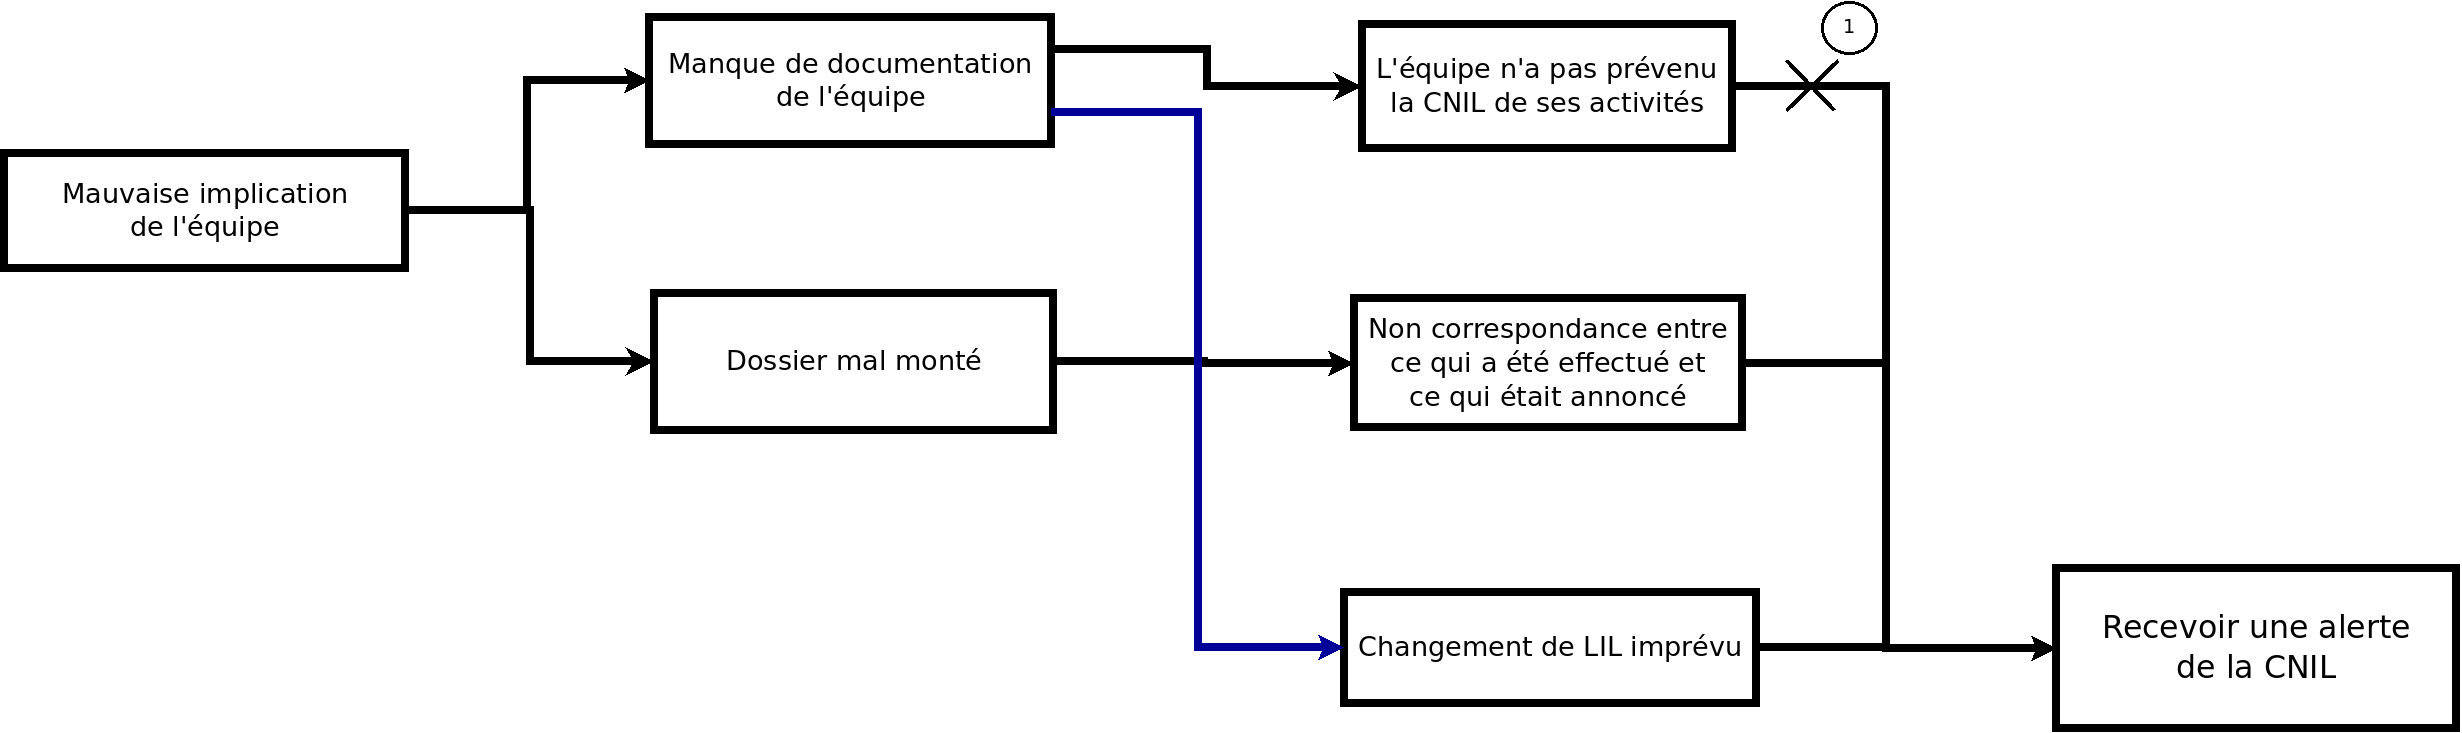
\includegraphics[scale=0.15]{images/AnalyseRisque_nPourquoi_FDR010}
	\caption{\label{risque pb cnil} Problème avec la CNIL - méthode des n pourquoi}
\end{figure}
\chapter*{Fiche de Risque 011}
% version 1.00	date 29/01/2016  	Auteur Sergi Colomies

\section*{Informations générales}
 
\begin{table}[H]
\centering
	\begin{tabularx}{16.8cm}{|X|X|}
	\hline
	\rowcolor{gray!40} Numéro du risque & Type du risque \\
	\hline
	011 & Retard de remise de données de la part du client \\
	\hline
	\end{tabularx}
\end{table}

\begin{table}[H]
\centering
	\begin{tabularx}{16.8cm}{|X|X|X|}
	\hline
	\rowcolor{gray!40} Date & Visa du \RQ & Visa du \CP \\
	\hline
	  &  &  \\
	\hline
	\end{tabularx}
\end{table}

\begin{table}[H]
\centering
	\begin{tabularx}{16.8cm}{|X|X|X|X|}
	\hline
	\rowcolor{gray!40} Pilote & Activité WBS & Compte WBS & Phase d'apparition \\
	\hline
	 \Sergi & Suivre les Risques et Opportunités & 1.2.3.2 & À tout moment\\
	\hline
	\end{tabularx}
\end{table}

\section*{Description du risque}

\subsection*{Résumé}
	Le risque lié au retard des données peut impacter sur la durée critique du projet. Celui-ci pourrait intervenir sur n'importe quel phase étant donnée que le terme donnée est ici générique.
	
\subsection*{Analyse des causes}
	voir figure \ref{risque retard data}.

\subsection*{Criticité}

\begin{table}[H]
\centering
	\begin{tabularx}{16.8cm}{|>{\columncolor{gray!40}}X|X|}
	\hline
	Gravité & 2\\
	\hline
	Probabilité & 2\\
	\hline
	Criticité & A surveiller \\
	\hline
	\end{tabularx}
\end{table}
\newpage

\section*{Actions}
\subsection*{Actions préventives}

%\begin{table}[H]
\centering
	\begin{longtable}{|p{7cm}|p{7cm}|}
	\hline
	\rowcolor{gray!40} Numéro de cause & Actions préventives \\
	\hline
	 1 & \begin{itemize}
	 	\item Demander un envoi de données de deux manières différentes
	 \end{itemize} \\
	\hline
	2 & \begin{itemize}
		\item Voir les actions préventives au risque associé 
	\end{itemize} \\
	\hline
	3 & \begin{itemize}
		\item Voir actions préventives pour le risque associé
	\end{itemize} \\
	\hline
	\end{longtable}
%\end{table}

\flushleft
\subsection*{Plan de contournement}

\begin{enumerate}
	\item Utiliser des données test en attendant un retour du client
\end{enumerate}

\section*{Décision de clôture}
Par le \CP{} et le pilote du risque.
\begin{table}[H]
\centering
	\begin{tabularx}{16.8cm}{|X|X|}
	\hline
	\rowcolor{gray!40} Date de clôture & Raison de la clôture \\
	\hline
	 14/03/2016 & Données reçues\\
	\hline
	\end{tabularx}
\end{table}

\section*{Historique des modifications}
\begin{table}[H]
\centering
	\begin{tabularx}{16.8cm}{|X|X|}
	\hline
	\rowcolor{gray!40} Date & Modification \\
	\hline
	 14/03/2016 & clôture \\
	\hline
	\end{tabularx}
\end{table}
\newpage

%\begin{landscape}
\begin{figure}
	\centering
	\includegraphics[scale=0.30]{images/AnalyseRisque_nPourquoi_FDR011}
	\caption{\label{risque retard data} Retard de remise des données - méthode des n pourquoi}
\end{figure}
%\end{landscape}
\chapter*{Fiche de Risque 012}
\section*{Informations générales}
 
\begin{table}[H]
\centering
	\begin{tabularx}{16.8cm}{|X|X|}
	\hline
	\rowcolor{gray!40} Numéro du risque & Type du risque \\
	\hline
	012 & Retard de remise du livrable au client \\
	\hline
	\end{tabularx}
\end{table}

\begin{table}[H]
\centering
	\begin{tabularx}{16.8cm}{|X|X|X|}
	\hline
	\rowcolor{gray!40} Date & Visa du \RQ & Visa du \CP \\
	\hline
	  &  &  \\
	\hline
	\end{tabularx}
\end{table}

\begin{table}[H]
\centering
	\begin{tabularx}{16.8cm}{|X|X|X|X|}
	\hline
	\rowcolor{gray!40} Pilote & Activité WBS & Compte WBS & Phase d'apparition \\
	\hline
	 \Kafui & Suivre les Risques et Opportunités & 1.2.3.2 & À tout moment\\
	\hline
	\end{tabularx}
\end{table}

\section*{Description du risque}

\subsection*{Résumé}
	Le risque lié au retard de remise du livrable au client pourrait considérablement impacter la notoriété de l'établissement et de l'équipe PIC . Ce risque pourrait aussi éventuellement impliquer sur les activités du client.
	
\subsection*{Analyse des causes}
	voir figure \ref{risque retard de remise du livrable}.

\subsection*{Criticité}

\begin{table}[H]
\centering
	\begin{tabularx}{16.8cm}{|>{\columncolor{gray!40}}X|X|}
	\hline
	Gravité & 4\\
	\hline
	Probabilité & 1\\
	\hline
	Criticité & Critique\\
	\hline
	\end{tabularx}
\end{table}
\newpage

\section*{Actions}
\subsection*{Actions préventives}

%\begin{table}[H]
\centering
	\begin{longtable}{|p{7cm}|p{7cm}|}
	\hline
	\rowcolor{gray!40} Numéro de cause & Actions préventives \\
	\hline
	 1 & \begin{itemize}
	 	\item Communiquer régulièrement avec le client.
	 	\item
	 	Prévoir des réunions à un rythme régulier
	 \end{itemize} \\
	\hline
	2 & \begin{itemize}
		\item Voir les actions préventives au risque associé 
	\end{itemize} \\
	\hline
	3 & \begin{itemize}
		\item Rechercher un support convenant à la fois au client et à l'équipe PIC.
	\end{itemize} \\
	\hline
	4 & \begin{itemize}
		\item Voir les actions préventives au risque associé 
	\end{itemize} \\
	\hline
	5 & \begin{itemize}
		\item S'assurer que chaque tâche soit réparti
à la personne approprié.
	\item
	S'assurer que chaque tâche soit réparti
à la personne approprié.
\item Maintenir les fiches de compétences à jour. 
\item Proposer une formation adéquat dans le cas où un manque se déclare.	
	
	\end{itemize} \\
	\hline
	\end{longtable}
%\end{table}

\flushleft
\subsection*{Plan de contournement}

\begin{enumerate}
	\item Utiliser des données test en attendant un retour du client
\end{enumerate}

\section*{Décision de clôture}
Par le \CP{} et le pilote du risque.
\begin{table}[H]
\centering
	\begin{tabularx}{16.8cm}{|X|X|}
	\hline
	\rowcolor{gray!40} Date de clôture & Raison de la clôture \\
	\hline
	  & \\
	\hline
	\end{tabularx}
\end{table}

\section*{Historique des modifications}
\begin{table}[H]
\centering
	\begin{tabularx}{16.8cm}{|X|X|}
	\hline
	\rowcolor{gray!40} Date & Modification \\
	\hline
	  & \\
	\hline
	\end{tabularx}
\end{table}
\newpage

\begin{figure}
	\centering
	\includegraphics[scale=0.35]{images/AnalyseRisque_nPourquoi_FDR012}
	\caption{\label{risque retard de remise du livrable} Retard de remise du livrable - méthode des n pourquoi}
\end{figure}

\chapter*{Fiche de Risque 013}
% version 1.01	date 14/03/2016  	Auteur Mélissa Bignoux Pierre Porche

\section*{Informations générales}

\begin{table}[H]
\centering
	\begin{tabularx}{16.8cm}{|X|X|}
	\hline
	\rowcolor{gray!40} Numéro du risque & Type du risque \\
	\hline
	013 & Le livrable ne fonctionne pas chez le client \\
	\hline
	\end{tabularx}
\end{table}

\begin{table}[H]
\centering
	\begin{tabularx}{16.8cm}{|X|X|X|}
	\hline
	\rowcolor{gray!40} Date & Visa du \RQ & Visa du \CP \\
	\hline
	 29/01/16 & pgpic & pgpic \\
	\hline
	\end{tabularx}
\end{table}

\begin{table}[H]
\centering
	\begin{tabularx}{16.8cm}{|X|X|X|X|}
	\hline
	\rowcolor{gray!40} Pilote & Activité WBS & Compte WBS & Phase d'apparition \\
	\hline
	 \Melissa & Suivre les Risques et Opportunités & 1.2.3.2 & Après la livraison de chaque livrable. \\
	\hline
	\end{tabularx}
\end{table}

\section*{Description du risque}

\subsection*{Résumé}
	Le risque lié au fonctionnement du livrable chez le client peut entraîner un produit final non fonctionnel et une insatisfaction du client.
	
\subsection*{Analyse des causes}
	voir figure \ref{livrable fonctionne pas client}.

\subsection*{Criticité}

\begin{table}[H]
\centering
	\begin{tabularx}{16.8cm}{|>{\columncolor{gray!40}}X|X|}
	\hline
	Gravité & 4\\
	\hline
	Probabilité & 4\\
	\hline
	Criticité & Critique \\
	\hline
	\end{tabularx}
\end{table}
\newpage

\section*{Actions}
\subsection*{Actions préventives}

%\begin{table}[H]
\centering
	\begin{longtable}{|p{7cm}|p{7cm}|}
	\hline
	\rowcolor{gray!40} Numéro de cause & Actions préventives \\
	\hline
	1 & \begin{itemize}
	 	\item Former le \RD 
	 	\item Vérification de la part du \CP{} et des développeurs
	 \end{itemize} \\
	\hline
	2 & \begin{itemize}
		\item Se renseigner sur l'équipement dont dispose les clients
	\end{itemize}	 \\
	\hline
	3 & \begin{itemize}
		\item Former le client à l'utilisation du produit
	\end{itemize} \\
	\hline
	4 & \begin{itemize}
		\item Voir les actions préventives associées à ce risque
	\end{itemize} \\
	\hline
	\end{longtable}
%\end{table}

\flushleft
\subsection*{Plan de contournement}

\begin{enumerate}
	\item Améliorer les tests. 
\end{enumerate}

\section*{Décision de clôture}
Par le \CP{} et le pilote du risque.
\begin{table}[H]
\centering
	\begin{tabularx}{16.8cm}{|X|X|}
	\hline
	\rowcolor{gray!40} Date de clôture & Raison de la clôture \\
	\hline
	  & \\
	\hline
	\end{tabularx}
\end{table}

\section*{Historique des modifications}
\begin{table}[H]
\centering
	\begin{tabularx}{16.8cm}{|X|X|}
	\hline
	\rowcolor{gray!40} Date & Modification \\
	\hline
	 11/04/2016 & probabilité augmentée car livrable peu stable \\
	\hline
	 14/03/2016 & modification criticité\\
	\hline
	 20/04/2016 & modification criticité\\
	\hline
	\end{tabularx}
\end{table}
\newpage


\begin{figure}
	\centering
	\includegraphics[scale=1.2]{images/nPourquoiFDR013}
	\caption{\label{livrable fonctionne pas client}risque livrable ne fonctionne pas chez le client - méthode des n pourquoi}
\end{figure}


%\chapter*{Fiche d'Opportunités 001}
%\section*{Informations générales}
 
\begin{table}[H]
\centering
	\begin{tabularx}{16.8cm}{|X|X|}
	\hline
	\rowcolor{gray!40} Numéro de l'opportunité & Type de l'opportunité \\
	\hline
	001 & Acquisition d'un serveur gratuit pour le livrable \\
	\hline
	\end{tabularx}
\end{table}

\begin{table}[H]
\centering
	\begin{tabularx}{16.8cm}{|X|X|X|}
	\hline
	\rowcolor{gray!40} Date & Visa du \RQ & Visa du \CP \\
	\hline
	 07/12/15 & pgpic & pgpic \\
	\hline
	\end{tabularx}
\end{table}

\begin{table}[H]
\centering
	\begin{tabularx}{16.8cm}{|X|X|X|X|}
	\hline
	\rowcolor{gray!40} Pilote & Activité WBS & Compte WBS & Phase d'apparition \\
	\hline
	 \Matthieu & Suivre les Risques et Opportunités & 1.2.3.2 & Dès le début du PIC\\
	\hline
	\end{tabularx}
\end{table}

\section*{Description de l'opportunité}

\subsection*{Résumé}
	L'opportunité lié à l'acquisition d'un serveur gratuit permettrait de pouvoir déployer notre livrable et de mettre en place le service pour le client, sans contrainte budgétaire.
	
\subsection*{Analyse des causes}
	voir figure.

\subsection*{Criticité}

\begin{table}[H]
\centering
	\begin{tabularx}{16.8cm}{|>{\columncolor{gray!40}}X|X|}
	\hline
	Bénéfice & 4\\
	\hline
	Probabilité & 1\\
	\hline
	Criticité & Important\\
	\hline
	\end{tabularx}
\end{table}
\newpage

\section*{Actions}
\subsection*{Actions proactives}

%\begin{table}[H]
\centering
	\begin{longtable}{|p{7cm}|p{7cm}|}
	\hline
	\rowcolor{gray!40} Numéro de cause & Actions préventives \\
	\hline
	 1 & \begin{itemize}
	 	\item Formation sur les démarches nécessaires à la constitution d'un dossier de mécénat
	 \end{itemize} \\
	\hline
	2 & \\
	\begin{itemize}
		\item Recherche d'un hébergeur
		\item Comparaison des offres
		\item Étudier leur susceptibilité à accepter un mécénat
	\end{itemize}
	\hline
	3 & \begin{itemize}
		\item Constitution d'un dossier de mécénat
	\end{itemize} \\
	\hline
	4 & \begin{itemize}
		\item Discuter de la possibilité avec l'unité P3
		\item Faire une demande auprès de l'INSA
	\end{itemize}
	\hline
	5 & \begin{itemize}
		\item Faire une demande de mécénat auprès de l'hébergeur
		\item Faire connaître l'Unicef à l'hébergeur (plaquette, etc.)
		\item Discuter des avantages pour l'hébergeur à accepter le mécénat
	\end{itemize} \\
	\hline
	6 & \begin{itemize}
		\item Faire une demande auprès de l'Unicef France
	\end{itemize} \\
	\hline
	\hline
	\end{longtable}
%\end{table}

\section*{Décision de clôture}
Par le \CP{} et le pilote du risque.
\begin{table}[H]
\centering
	\begin{tabularx}{16.8cm}{|X|X|}
	\hline
	\rowcolor{gray!40} Date de clôture & Raison de la clôture \\
	\hline
	  & \\
	\hline
	\end{tabularx}
\end{table}

\section*{Historique des modifications}
\begin{table}[H]
\centering
	\begin{tabularx}{16.8cm}{|X|X|}
	\hline
	Date & Modification \\
	\hline
	  & \\
	\hline
	\end{tabularx}
\end{table}
\newpage

\begin{landscape}
\begin{figure}
	\centering
	\includegraphics[scale=0.35]{images/AnalyseRisque_nPourquoi_FDO001.png}
\end{figure}
\end{landscape}
\chapter*{Fiche d'Opportunités 002}
% version 1.01	date 14/03/2016  	Auteur Kafui Atanley Pierre Porche

\section*{Informations générales}
 
\begin{table}[H]
\centering
	\begin{tabularx}{16.8cm}{|X|X|}
	\hline
	\rowcolor{gray!40} Numéro de l'opportunité & Type de l'opportunité \\
	\hline
	 002 & Livrable terminé en avance  \\
	\hline
	\end{tabularx}
\end{table}

\begin{table}[H]
\centering
	\begin{tabularx}{16.8cm}{|X|X|X|}
	\hline
	\rowcolor{gray!40} Date & Visa du \RQ & Visa du \CP \\
	\hline
	 29/01/2016 & pgpic & pgpic \\
	\hline
	\end{tabularx}
\end{table}

\begin{table}[H]
\centering
	\begin{tabularx}{16.8cm}{|X|X|X|X|}
	\hline
	\rowcolor{gray!40} Pilote & Activité WBS & Compte WBS & Phase d'apparition \\
	\hline
	 \Kafui & Suivre les Risques et Opportunités & 1.2.3.2 & Fin de Sprint \\
	\hline
	\end{tabularx}
\end{table}

\section*{Description de l'opportunité}

\subsection*{Résumé}
	Le livrable disponible à l'avance permettrait de passer directement à la phase de recette. Ceci permettrait de réinvestir le temps gagné dans une autre phase.
	
\subsection*{Analyse des causes}
	
Voir figure \ref{opportunite livrable termine en avance}.

\subsection*{Criticité}

\begin{table}[H]
\centering
	\begin{tabularx}{16.8cm}{|>{\columncolor{gray!40}}X|X|}
	\hline
	Bénéfice & 4\\
	\hline
	Probabilité & 1 \\
	\hline
	Criticité & Important \\
	\hline
	\end{tabularx}
\end{table}

\newpage
\section*{Actions}
\subsection*{Actions proactives}

{\centering
	\begin{longtable}{|p{7cm}|p{7cm}|}
	\hline
	\rowcolor{gray!40}Numéro de cause & Actions proactives \\
	
	\hline
	  1 &  \begin{itemize}
	  	\item Entretien individualisé
	  	\item Bonne communication
	  	\end{itemize} \\
	  	
	  \hline
	  2 & \begin{itemize} 
	  \item Team-Building
	  \item Entretien individualisé
	  \end{itemize} \\
	  \hline
	  3 & \begin{itemize} 
	  \item Faire remonter les problématiques fréquentes rencontrées en PIC à la direction. 
	  \end{itemize} \\
	  \hline
	   4 & \begin{itemize}
	   \item Bonne communication autour du projet. 
	   \end{itemize} \\
	\hline
	
\end{longtable}}

\section*{Décision de clôture}
Par le \CP{} et le pilote du risque.
\begin{table}[h]
\centering
	\begin{tabularx}{16.8cm}{|X|X|}
	\hline
	\rowcolor{gray!40} Date de clôture & Raison de la clôture \\
	\hline
	  & \\
	\hline
	\end{tabularx}
\end{table}

\section*{Historique des modifications}
\begin{table}[h]
\centering
	\begin{tabularx}{16.8cm}{|X|X|}
	\hline
	\rowcolor{gray!40} Date & Modification \\
	\hline
	 14/03/2016 & modifications criticité \\
	\hline
	\end{tabularx}
\end{table}
\newpage

\begin{figure}[!h]
	\centering
	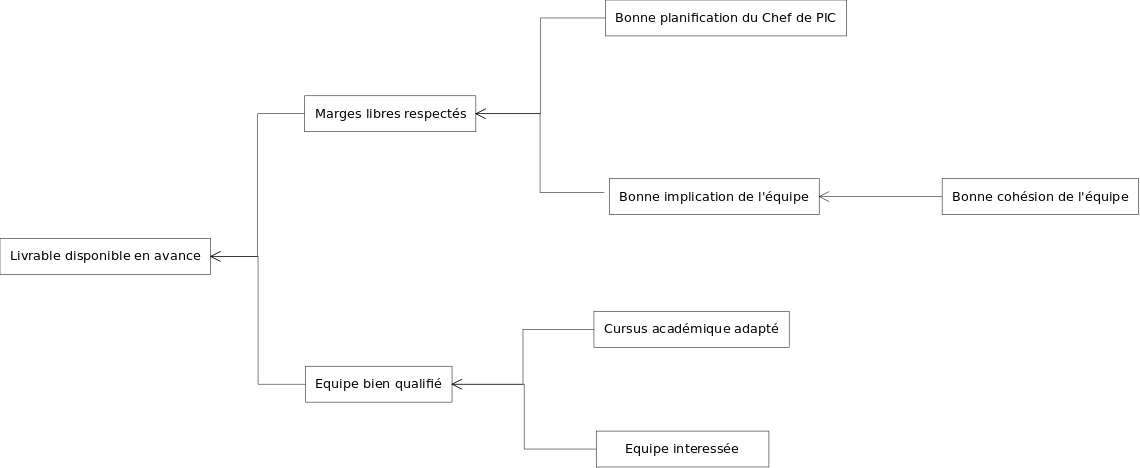
\includegraphics[scale=0.27]{images/AnalyseOpportunite_nPourquoi_FDO002}
	\caption{\label{opportunite livrable termine en avance} Opportunité livrable terminé en avance - méthode des n pourquoi}
\end{figure}

\chapter*{Fiche d'Opportunités 003}
% version 1.01, date 14/03/16, auteur Pierre Porche
\section*{Informations générales}
 
\begin{table}[h]
\centering
	\begin{tabularx}{16.8cm}{|X|X|}
	\hline
	\rowcolor{gray!40} Numéro de l'opportunité & Type d'opportunité \\
	\hline
	003 & Bonne passation \\
	\hline
	\end{tabularx}
\end{table}

\begin{table}[h]
\centering
	\begin{tabularx}{16.8cm}{|X|X|X|}
	\hline
	\rowcolor{gray!40} Date & Visa du \RQ & Visa du \CP \\
	\hline
	 29/01/2016 & pgpic & pgpic \\
	\hline
	\end{tabularx}
\end{table}

\begin{table}[h]
\centering
	\begin{tabularx}{16.8cm}{|X|X|X|X|}
	\hline
	\rowcolor{gray!40} Pilote & Activité WBS & Compte WBS & Phase d'apparition \\
	\hline
	 \Francois & Suivre les Risques et Opportunités & 1.2.3.2 & A partir de la fin du premier semestre.\\
	\hline
	\end{tabularx}
\end{table}

\section*{Description de l'opportunité}

\subsection*{Résumé}
	Grâce à une bonne passation, le temps de prise en main du projet par la nouvelle équipe pourrait être grandement réduit.
	
\subsection*{Analyse des causes}
	voir figure \ref{opportunite bonne passation}.

\subsection*{Criticité}

\begin{table}[h]
\centering
	\begin{tabularx}{16.8cm}{|>{\columncolor{gray!40}}X|X|}
	\hline
	Bénéfice & 3\\
	\hline
	Probabilité & 2\\
	\hline
	Criticité & Moyen \\
	\hline
	\end{tabularx}
\end{table}
\newpage

\section*{Actions}
\subsection*{Actions proactives}

%\begin{table}[H]
{\centering
	\begin{longtable}{|p{7cm}|p{7cm}|}
	\hline
	\rowcolor{gray!40} Cause & Actions proactives \\
	\hline
	 Rédaction de documents de passation & \begin{itemize}
	 	\item Attribuer cette tâche
	 	\item Inclure cette tâche dans le planning
	 	\item Commencer cette tâche à temps
	 \end{itemize} \\
	\hline
	Arrivée de la nouvelle équipe avant départ de l'ancienne & \begin{itemize}
		\item Demander à la nouvelle équipe d'arriver au plus tôt
	\end{itemize} \\
	\hline
	Communication préalable avec la nouvelle équipe & \begin{itemize}
		\item Organiser des rendez-vous téléphoniques
		\item Prévenir la nouvelle équipe de ces rendez-vous
	\end{itemize} \\
	\hline
	Passation prévue et organisée & \begin{itemize}
		\item Réfléchir au processus de passation
		\item Inclure la préparation de la passation dans le planning
		\item Nommer un responsable de la passation
	\end{itemize} \\
	\hline
	Mise en place d'outils de communication performants & \begin{itemize}
		\item Rechercher les outils les plus adaptés
		\item Tester différents outils
	\end{itemize} \\
	\hline
	Bonne planification & \begin{itemize}
		\item Former le \CP à la planification
		\item Bien prévoir les temps nécessaires à chaque tâche
	\end{itemize} \\
	\hline

	\end{longtable}}
%\end{table}


\section*{Décision de clôture}
Par le \CP{} et le pilote du risque.
\begin{table}[h]
\centering
	\begin{tabularx}{16.8cm}{|X|X|}
	\hline
	\rowcolor{gray!40} Date de clôture & Raison de la clôture \\
	\hline
	 19/10/2016 & clôture \\
	\hline
	\end{tabularx}
\end{table}

\section*{Historique des modifications}
\begin{table}[h]
\centering
	\begin{tabularx}{16.8cm}{|X|X|}
	\hline
	\rowcolor{gray!40} Date & Modification \\%\rowcolor{gray!40}
	\hline
	 21/09/2016 & clôture \\ 
	\hline
	 06/09/2016 & modification pilote car changement d'équipe \\
	\hline
	 14/03/2016 & modifications criticité \\
	\hline
	\end{tabularx}
\end{table}
\newpage


\begin{figure}
	\centering
	\includegraphics[scale=0.5]{images/nPourquoiFDO003}
	\caption{\label{opportunite bonne passation}Opportunité bonne passation - méthode des n pourquoi}
\end{figure}

\chapter*{Fiche d'Opportunités 004}
% version 1.01	Auteur Florian Leriche Pierre Porche

\section*{Informations générales}
 
\begin{table}[h]
\centering
	\begin{tabularx}{16.8cm}{|X|X|}
	\hline
	\rowcolor{gray!40} Numéro de l'opportunité & Type d'opportunité \\
	\hline
	004 & Bonne communication client \\
	\hline
	\end{tabularx}
\end{table}

\begin{table}[h]
\centering
	\begin{tabularx}{16.8cm}{|X|X|X|}
	\hline
	 \rowcolor{gray!40} Date & Visa du \RQ & Visa du \CP \\
	\hline
	 29/01/2016 & pgpic & pgpic \\
	\hline
	\end{tabularx}
\end{table}

\begin{table}[h]
\centering
	\begin{tabularx}{16.8cm}{|X|X|X|X|}
	\hline
	\rowcolor{gray!40} Pilote & Activité WBS & Compte WBS & Phase d'apparition \\
	\hline
	 \Florian & Suivre les Risques et Opportunités & 1.2.3.2 & Tout au long du projet.\\
	\hline
	\end{tabularx}
\end{table}

\section*{Description du risque}

\subsection*{Résumé}
	Une bonne communication avec le client peut entraîner une meilleure compréhension de ses besoins. Cela peut permettre à l'équipe \PICCourt de mieux répondre aux exigences du client et d'éviter d'éventuels retards dans les livraisons. \\
        La bonne communication avec le client peut être due à une bonne gestion des différents outils de communication ou une bonne réactivité de sa part.
	
\subsection*{Analyse des causes}
	voir figure \ref{opportunite bonne communication client}.

\subsection*{Criticité}

\begin{table}[h]
\centering
	\begin{tabularx}{16.8cm}{|>{
	\columncolor{gray!40}
	}X|X|}
	\hline
	Bénéfice & 3\\
	\hline
	Probabilité & 4\\
	\hline
	Criticité & Important\\
	\hline
	\end{tabularx}
\end{table}
\newpage

\section*{Actions}
\subsection*{Actions proactives}

%\begin{table}[H]
{\centering
	\begin{longtable}{|p{7cm}|p{7cm}|}
	\hline
	\rowcolor{gray!40} Cause & Actions proactives \\
	\hline
	 Se faire comprendre par le client & \begin{itemize}
	 	\item S'adapter aux connaissances du client.
	 	\item Ne pas employer de vocabulaire trop spécifique.
	 \end{itemize} \\
	\hline
	Respecter ses engagements et promesses & \begin{itemize}
		\item Ne pas se surestimer.
		\item Être franc avec le client.
	\end{itemize} \\
	\hline
	Bonne gestion des outils de communication & \begin{itemize}
		\item Désigner un responsable de ces différents outils.
	\end{itemize} \\
	\hline
	Gérer sa communication & \begin{itemize}
		\item Ne pas se précipiter.
		\item Se maîtriser et se préparer.
	\end{itemize} \\
	\hline
	Choix pertinents des outils de communication & \begin{itemize}
		\item Rechercher les outils les plus adaptés.
		\item Tester différents outils.
	\end{itemize} \\
	\hline
	Bonne maîtrise des outils de communication & \begin{itemize}
		\item Former les membres de l'équipe à l'utilisation des ces outils
	\end{itemize} \\
	\hline
	Être proche du client & \begin{itemize}
		\item Prendre contact régulièrement avec le client.
		\item Prendre en compte les remarques du client.
	\end{itemize} \\
	\hline
	Mise en place d'outils de communication performants & \begin{itemize}
		\item Rechercher les outils les plus adaptés
		\item Tester différents outils
	\end{itemize} \\
	\hline
	\end{longtable}}
%\end{table}

\section*{Décision de clôture}
Par le \CP{} et le pilote du risque.
\begin{table}[h]
\centering
	\begin{tabularx}{16.8cm}{|X|X|}
	\hline
	\rowcolor{gray!40} Date de clôture & Raison de la clôture \\
	\hline
	  & \\
	\hline
	\end{tabularx}
\end{table}

\section*{Historique des modifications}
\begin{table}[h]
\centering
	\begin{tabularx}{16.8cm}{|X|X|}
	\hline
	\rowcolor{gray!40} Date & Modification \\%\rowcolor{gray!40} 
	\hline
	 14/03/2016 & criticité \\
	\hline
	\end{tabularx}
\end{table}
\newpage


\begin{figure}
	\centering
	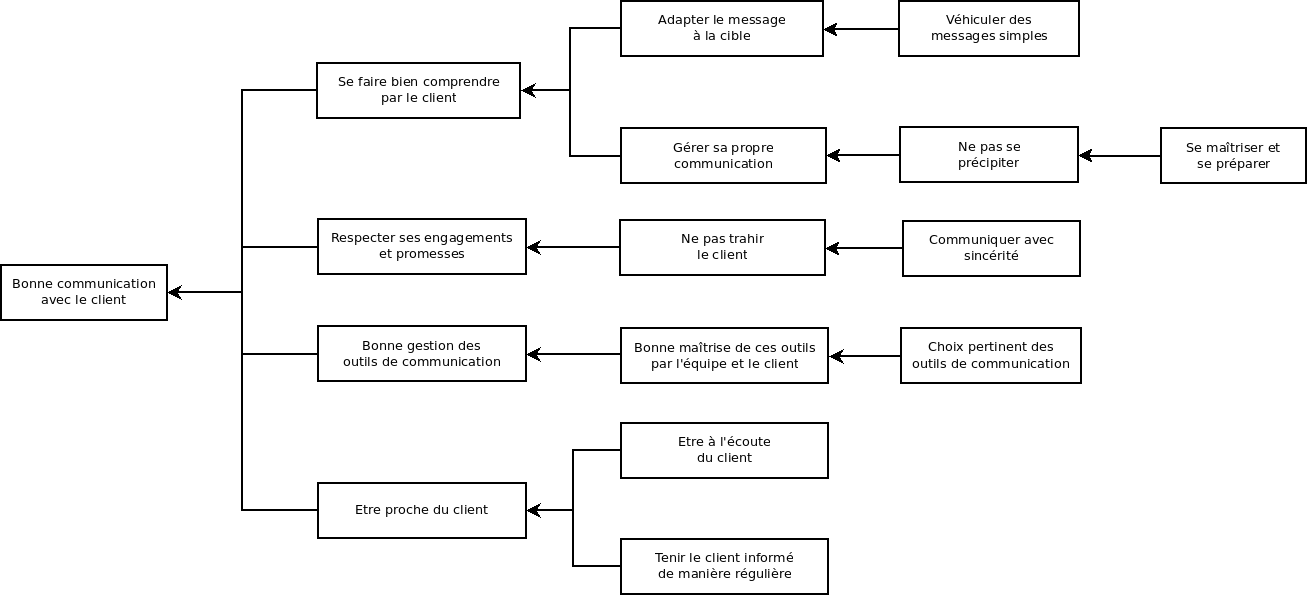
\includegraphics[scale=0.28]{images/AnalyseOpportunite_nPourquoi_FDO004}
	\caption{\label{opportunite bonne communication client}Opportunité bonne communication client - méthode des n pourquoi}
\end{figure}

\chapter*{Fiche d'Opportunités 005}
% version 1.01	Auteur Florian Leriche Pierre Porche

\section*{Informations générales}
 
\begin{table}[h]
\centering
	\begin{tabularx}{16.8cm}{|X|X|}
	\hline
	\rowcolor{gray!40} Numéro de l'opportunité & Type d'opportunité \\
	\hline
	005 & Bonne planification \\
	\hline
	\end{tabularx}
\end{table}

\begin{table}[h]
\centering
	\begin{tabularx}{16.8cm}{|X|X|X|}
	\hline
	\rowcolor{gray!40} Date & Visa du \RQ & Visa du \CP \\
	\hline
	 29/01/2016 & pgpic & pgpic \\
	\hline
	\end{tabularx}
\end{table}

\begin{table}[h]
\centering
	\begin{tabularx}{16.8cm}{|X|X|X|X|}
	\hline
	\rowcolor{gray!40} Pilote & Activité WBS & Compte WBS & Phase d'apparition \\
	\hline
	 \Sergi & Suivre les Risques et Opportunités & 1.2.3.2 & Tout au long du projet.\\
	\hline
	\end{tabularx}
\end{table}

\section*{Description de l'opportunité}

\subsection*{Résumé}

	La bonne planification concerne principalement l’appréciation des délais des tâches
et peut être expliquée par une bonne implication du \CP. Elle permet de ne pas prendre de retard de
livraison des lots.
	
\subsection*{Analyse des causes}
	voir figure \ref{opportunite bonne planification}.

\subsection*{Criticité}

\begin{table}[h]
\centering
	\begin{tabularx}{16.8cm}{|>{\columncolor{gray!40}}X|X|}
	\hline
	Bénéfice & 3\\
	\hline
	Probabilité & 2\\
	\hline
	Criticité & Moyen \\
	\hline
	\end{tabularx}
\end{table}
\newpage

\section*{Actions}
\subsection*{Actions proactives}

%\begin{table}[H]
{\centering
	\begin{longtable}{|p{7cm}|p{7cm}|}
	\hline
	\rowcolor{gray!40}Cause & Actions proactives \\
	\hline
	 Choix des outils de plannification pertinent & \begin{itemize}
	 	\item 
	 \end{itemize} \\
	\hline
        Bonne prise en main des outils & \begin{itemize}
	 	\item Former les membres de l'équipe \PICCourt{}.
	 \end{itemize} \\
	\hline
        Bonne vision globale & \begin{itemize}
	 	\item Avoir un \CP{} impliqué et compétent.
	 \end{itemize} \\
	\hline
	\end{longtable}}
%\end{table}

\section*{Décision de clôture}
Par le \CP{} et le pilote du risque.
\begin{table}[h]
\centering
	\begin{tabularx}{16.8cm}{|X|X|}
	\hline
	\rowcolor{gray!40} Date de clôture & Raison de la clôture \\
	\hline
	  & \\
	\hline
	\end{tabularx}
\end{table}

\section*{Historique des modifications}
\begin{table}[h]
\centering
	\begin{tabularx}{16.8cm}{|X|X|}
	\hline
	\rowcolor{gray!40} Date & Modification \\%\rowcolor{gray!40} 
	\hline
	 14/03/2016 & criticité\\
	\hline
	\end{tabularx}
\end{table}
\newpage


\begin{figure}
	\centering
	\includegraphics[scale=0.5]{images/nPourquoiFDO005}
	\caption{\label{opportunite bonne planification}Opportunité bonne planification - méthode des n pourquoi}
\end{figure}

\chapter*{Fiche d'Opportunités 006}
% version 1.01, date 14/03/16, auteur Michel Cressant Pierre Porche
\section*{Informations générales}
 
\begin{table}[h]
\centering
	\begin{tabularx}{16.8cm}{|X|X|}
	\hline
	\rowcolor{gray!40} Numéro de l'opportunité & Type d'opportunité \\
	\hline
	006 & Bonne ambiance \\
	\hline
	\end{tabularx}
\end{table}

\begin{table}[h]
\centering
	\begin{tabularx}{16.8cm}{|X|X|X|}
	\hline
	\rowcolor{gray!40} Date & Visa du \RQ & Visa du \CP \\
	\hline
	 29/01/2016 & pgpic & pgpic \\
	\hline
	\end{tabularx}
\end{table}

\begin{table}[h]
\centering
	\begin{tabularx}{16.8cm}{|X|X|X|X|}
	\hline
	\rowcolor{gray!40} Pilote & Activité WBS & Compte WBS & Phase d'apparition \\
	\hline
	 \Michel & Suivre les Risques et Opportunités & 1.2.3.2 & Tout au long du projet.\\
	\hline
	\end{tabularx}
\end{table}

\section*{Description de l'opportunité}

\subsection*{Résumé}
	Une bonne ambiance au sein de l'équipe PIC permettrait d'augmenter considérablement la productivité des membres. \\
	
\subsection*{Analyse des causes}
	voir figure \ref{opportunite bonne ambiance}.

\subsection*{Criticité}

\begin{table}[h]
\centering
	\begin{tabularx}{16.8cm}{|>{\columncolor{gray!40}}X|X|}
	\hline
	Bénéfice & 3\\
	\hline
	Probabilité & 4\\
	\hline
	Criticité & Important \\
	\hline
	\end{tabularx}
\end{table}
\newpage

\section*{Actions}
\subsection*{Actions proactives}

%\begin{table}[H]
{\centering
	\begin{longtable}{|p{7cm}|p{7cm}|}
	\hline
 	\rowcolor{gray!40} Cause & Actions proactives \\
	\hline
	 Bonne communication & \begin{itemize}
	 	\item Maintenir un rythme régulier de réunions collectives.
	 	\item Mettre en place des entretiens individuels.
	 	\item Mettre en place du team-building.
	 \end{itemize} \\
	\hline
	Equipe impliquée dans le projet & \begin{itemize}
		\item Mettre en place du team-building.
	\end{itemize} \\
	\hline
	Bonne planification & \begin{itemize}
		\item Mettre les indicateurs à jour.
		\item Effectuer un suivi régulier du travail des membres.
	\end{itemize} \\
	\hline
	\end{longtable}}
%\end{table}

\section*{Décision de clôture}
Par le \CP{} et le pilote du risque.
\begin{table}[h]
\centering
	\begin{tabularx}{16.8cm}{|X|X|}
	\hline
	\rowcolor{gray!40} Date de clôture & Raison de la clôture \\
	\hline
	  & \\
	\hline
	\end{tabularx}
\end{table}

\section*{Historique des modifications}
\begin{table}[h]
\centering
	\begin{tabularx}{16.8cm}{|X|X|}
	\hline
	\rowcolor{gray!40} Date & Modification \\%\rowcolor{gray!40} 
	\hline
	14/03/2016  & criticité \\
	\hline
	\end{tabularx}
\end{table}
\newpage


\begin{figure}
	\centering
	\includegraphics[scale=0.35]{images/nPourquoiFDO006}
	\caption{\label{opportunite bonne ambiance}Opportunité bonne ambiance - méthode des n pourquoi}
\end{figure}
\chapter*{Fiche d'Opportunités 007}
\section*{Informations générales}
 
\begin{table}[H]
\centering
	\begin{tabularx}{16.8cm}{|X|X|}
	\hline
	\rowcolor{gray!40} Numéro du risque & Type du risque \\
	\hline
	007 &  Remise des données en avance \\
	\hline
	\end{tabularx}
\end{table}

\begin{table}[H]
\centering
	\begin{tabularx}{12.8cm}{|X|X|X|}
	\hline
	\rowcolor{gray!40} Date & Visa du \RQ & Visa du \CP \\
	\hline
	 07/12/15 & pgpic & pgpic \\
	\hline
	\end{tabularx}
\end{table}

\begin{table}[H]
\centering
	\begin{tabularx}{12.8cm}{|X|X|X|X|}
	\hline
	\rowcolor{gray!40} Pilote & Activité WBS & Compte WBS & Phase d'apparition \\
	\hline
	 \Sergi & Suivre les Risques et Opportunités & 1.2.3.2 & À partir de l’installation serveur\\
	\hline
	\end{tabularx}
\end{table}

\section*{Description du risque}

\subsection*{Résumé}
	La possibilité de recevoir les données du client en avance 
	
\subsection*{Analyse des causes}
	voir figure.

\subsection*{Criticité}

\begin{table}[H]
\centering
	\begin{tabularx}{12.8cm}{|>{\columncolor{gray!40}}X|X|}
	\hline
	Gravité & 2\\
	\hline
	Probabilité & 3\\
	\hline
	Criticité & Critique\\
	\hline
	\end{tabularx}
\end{table}
\newpage

\section*{Actions}
\subsection*{Actions proactives}

%\begin{table}[H]
\centering
	\begin{longtable}{|p{7cm}|p{7cm}|}
	\hline
	\rowcolor{gray!40} Nom de cause & Actions proactives \\
	\hline
	 1 & \begin{itemize}
	 	\item Boîte à idée
	 	\item Faire des tickets
	 	\item Réunions fréquentes
	 	\item Laisser la parole à tout le monde
	 	\item Hiérarchie bien définie
	 	\item Choisir les bons outils
	 	\item Faire des compte rendus de réunion à envoyer au client
	 	\item Être en constante délibération
	 	\item Reformulation des spécifications
	 	\item Avoir un interlocuteur unique entre le client et le \PICCourt
	 	\item Suivi hebdomadaire de l'avancement
	 \end{itemize} \\
	\hline
	2 & \\
	\hline
	3 & \begin{itemize}
		\item Choisir de bonnes valeurs seuils
		\item Présence et assiduité
		\item Créneau horaire respecté
		\item Objectifs personnels
	\end{itemize} \\
	\hline
	4 & \begin{itemize}
		\item La personne qui fait les tests doit être différente de celle qui code
		\item Faire un maximum de tests
		\item Définir clairement les méthodes de travail dès le début du \PICCourt et faire vérifier par un référent
	\end{itemize} \\
	\hline
	5 & \begin{itemize}
		\item Se former sur la réalisation d'un audit sécurité
		\item Effectuer régulièrement des audits sécurité
		\item Nommer un responsable sécurité
		\item Faire des tests en boîte noire et boîte blanche
	\end{itemize} \\
	\hline
	6 & \begin{itemize}
		\item Faire les démarches nécessaires
		\item Être économe
		\item Faire un calcul du budget au début
	\end{itemize} \\
	\hline
	7 & \begin{itemize}
		\item Faire un planning
		\item Faire un GANTT/PERT
		\item Chacun respecte son rôle
		\item Bien définir les rôles
		\item Faire des réunions fréquentes
		\item Utiliser les bons outils de partage
	\end{itemize} \\
	\hline
	8 & \begin{itemize}
		\item Avoir une méthode de paiement de secours
		\item Se renseigner auprès des prestataires
		\item Demander au département les méthodes de paiement autorisées
	\end{itemize} \\
	\hline
	9 & \begin{itemize}
		\item Former un bénévole
	\end{itemize} \\
	\hline
	10 & \begin{itemize}
		\item Actions de prévention et de formation
		\item Effectuer des sauvegardes régulières
	\end{itemize} \\
	\hline
	\end{longtable}
%\end{table}

\flushleft

\section*{Décision de clôture}
Par le \CP{} et le pilote du risque.
\begin{table}[H]
\centering
	\begin{tabularx}{16.8cm}{|X|X|}
	\hline
	\rowcolor{gray!40} Date de clôture & Raison de la clôture \\
	\hline
	  & \\
	\hline
	\end{tabularx}
\end{table}

\section*{Historique des modifications}
\begin{table}[H]
\centering
	\begin{tabularx}{16.8cm}{|X|X|}
	\hline
	Date & Modification \\
	\hline
	  & \\
	\hline
	\end{tabularx}
\end{table}
\newpage

\begin{landscape}
\begin{figure}
	\centering
	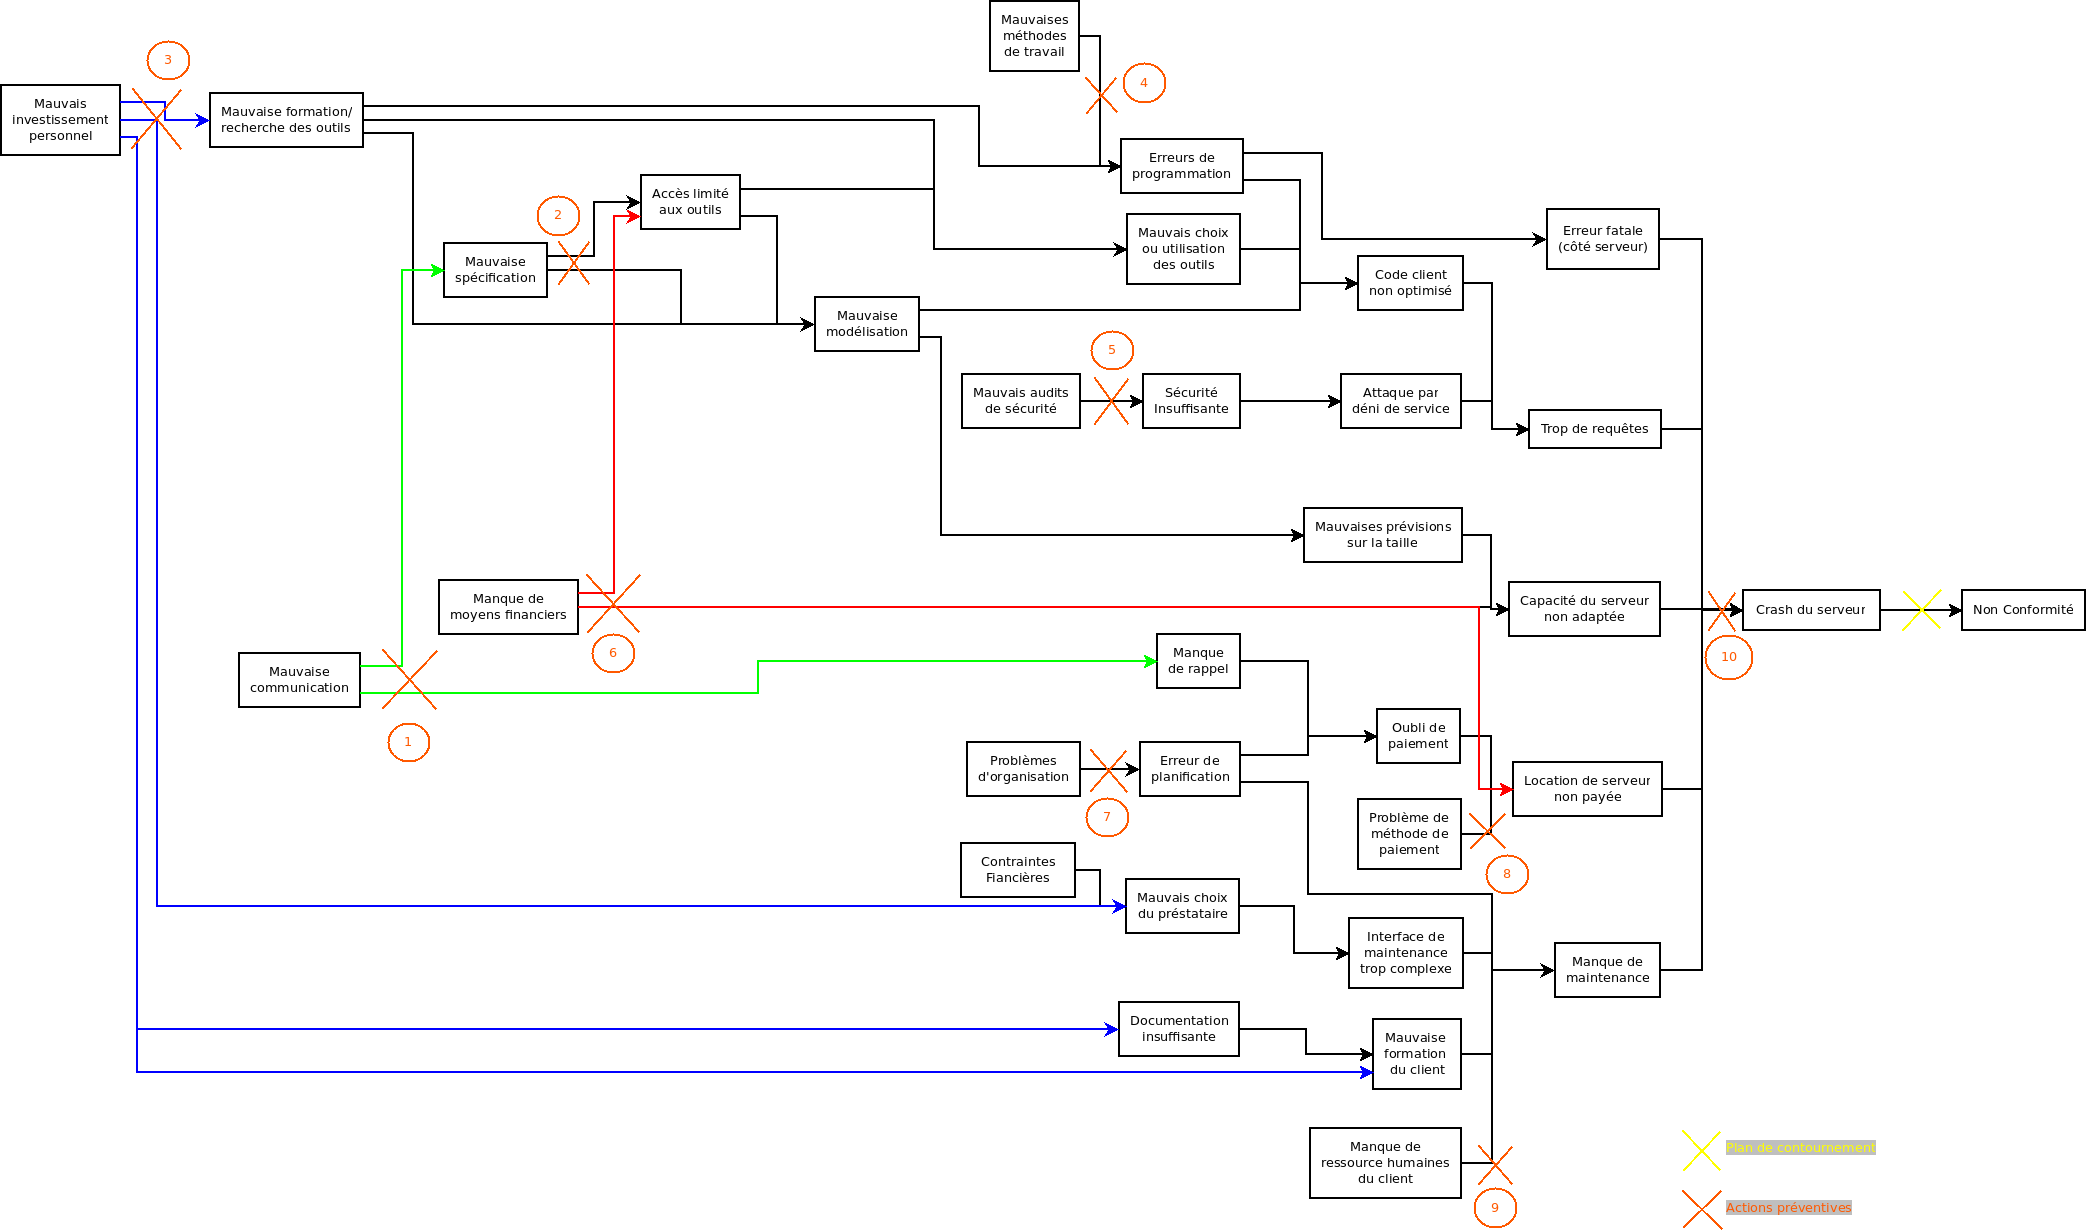
\includegraphics[scale=0.35]{images/AnalyseRisque_nPourquoi_FDR001.png}
\end{figure}
\end{landscape}





\chapter*{Suivi des Risques}
\begin{longtable}{|p{0.3cm}|p{2.5cm}|p{2cm}|p{2cm}|p{1.8cm}|p{1.5cm}|p{1cm}|p{1cm}|p{1.5cm}|}
			\hline
			\rowcolor{gray!40}
			\No & Nom & Pilote & Probabilité & Impact & Priorité & Visa \RQCourt{} & Visa \CPCourt{} & Clôture \\\hline
			 1 & Crash du serveur & \Matthieu & Peu probable & Maximum & Critique & pgpic & pgpic & \\\hline
			 2 & Mauvaise ambiance interne & \Michel & Possible & Important & À surveiller & pgpic & pgpic & \\\hline
			 3 & Abscebce collective & \Pierre & Peu probable & Maximum & Critique & pgpic & pgpic & \\\hline
			 4 & Mauvaise communication client & \Julie & Probable & Important & Critique & pgpic & pgpic & \\\hline
			 5 & Mauvaise planification & \Florian & Possible & Important & À surveiller & pgpic & pgpic & \\\hline
			 6 & Mauvaise mise en route du second semestre & \Melissa & Probable & Important & Critique & pgpic & pgpic & \\\hline
			 7 & Perte de documents & \Mathieu & Peu probable & Maximum & Critique & pgpic & pgpic & \\\hline
			 8 & Indisponibilité du client pour la remise des recettes & \Julie & possible & important & À surveiller & pgpic & pgpic & \\\hline
			 9 & Serveur extérieur non trouvé & \Matthieu & Probable & Maximum & Critique & pgpic & pgpic & \\\hline
			 10 & Problème avec la CNIL & \Pierre & Possible & Important & À surveiller & pgpic & pgpic & \\\hline
			 11 & Retard de remise des données & \Sergi & Possible & Moyen & À surveiller & pgpic & pgpic & \\\hline
			 12 & Retard de remise du livrable & \Kafui & Possible & Important & À surveiller & pgpic & pgpic & \\\hline
			 13 & Le livrable ne fonctionne pas chez le client & \Melissa & Peu probable & Important & À surveiller & pgpic & pgpic & \\\hline
\end{longtable}

\chapter*{Suivi des Opportunités}

\begin{longtable}{|p{0.3cm}|p{2.5cm}|p{2cm}|p{2cm}|p{1.8cm}|p{1.5cm}|p{1cm}|p{1cm}|p{1.5cm}|}
			\hline
			\rowcolor{gray!40}
			\No & Nom & Pilote & Probabilité & Impact & Priorité & Visa \RQCourt{} & Visa \CPCourt{} & Clôture \\\hline
			 1 & Serveur gratuit & \Matthieu & Peu probable & Maximum & Important & pgpic & pgpic & \\\hline
			 2 & Livrable terminé en avance & \Kafui & Possible & Maximum & Important & pgpic & pgpic & \\\hline
			 3 & Bonne passation inter-semestre & \Pierre & Probable & Important & Important & pgpic & pgpic & \\\hline
			 4 & Bonne communication client & \Florian & Probable & Important & Important & pgpic & pgpic & \\\hline
			 5 & Bonne planification & \Pierre & Très probable & Important & Important & pgpic & pgpic & \\\hline
			 6 & Bonne ambiance interne & \Michel & Très probable & Moyen & Important & pgpic & pgpic & \\\hline
			 7 & Remise des données en avance & \Sergi & Probable & Moyen & Moyen & pgpic & pgpic &  \\\hline
\end{longtable}

\end{document}